\section{Analysis of the \texorpdfstring{\ttH}{ttH} mode}
\label{sec:htoinv_analysis_ttH}

% Describe the specifics of the background estimation and fit for the ttH subcategories, since they may differ for the other modes, e.g.,
%   - Photon CR is not used for ttH. Dilepton CRs are aggregated over all boosted categories for statistical power and the rate parameter is left floating, being constrained by all ttH boosted subcategories and MET bins. Could try to explicitly write out how the CR likelihood functions evolve
%   - For QCD background estimation: "For the \ttH category, the tight double sideband from Tab.~\ref{tab:sideband_defs}---the most enriched in \acrshort{qcd} \acrshort{mc}---is used to derive \catFraction. The loose double sideband is used to derive \metFraction. This sideband is used for the prediction as a whole, i.e., for the terms $N_{\mathrm{SB}}^{\mathrm{QCD}}$ and $\transfac_{\mathrm{QCD}}$ in Eq.~\ref{eq:qcd_prediction}."
% Need to mention somewhere that the observed limit is given at 95% CL

Fig.~\ref{fig:htoinv_limit_ttH} showcases the median expected limit on $\BRof{\higgstoinv}$ with 1$\sigma$ and 2$\sigma$ bounds for the \ttH category and its subcategories.

\begin{figure}[htbp]
    \centering
    \begin{subfigure}[b]{0.45\textwidth}
        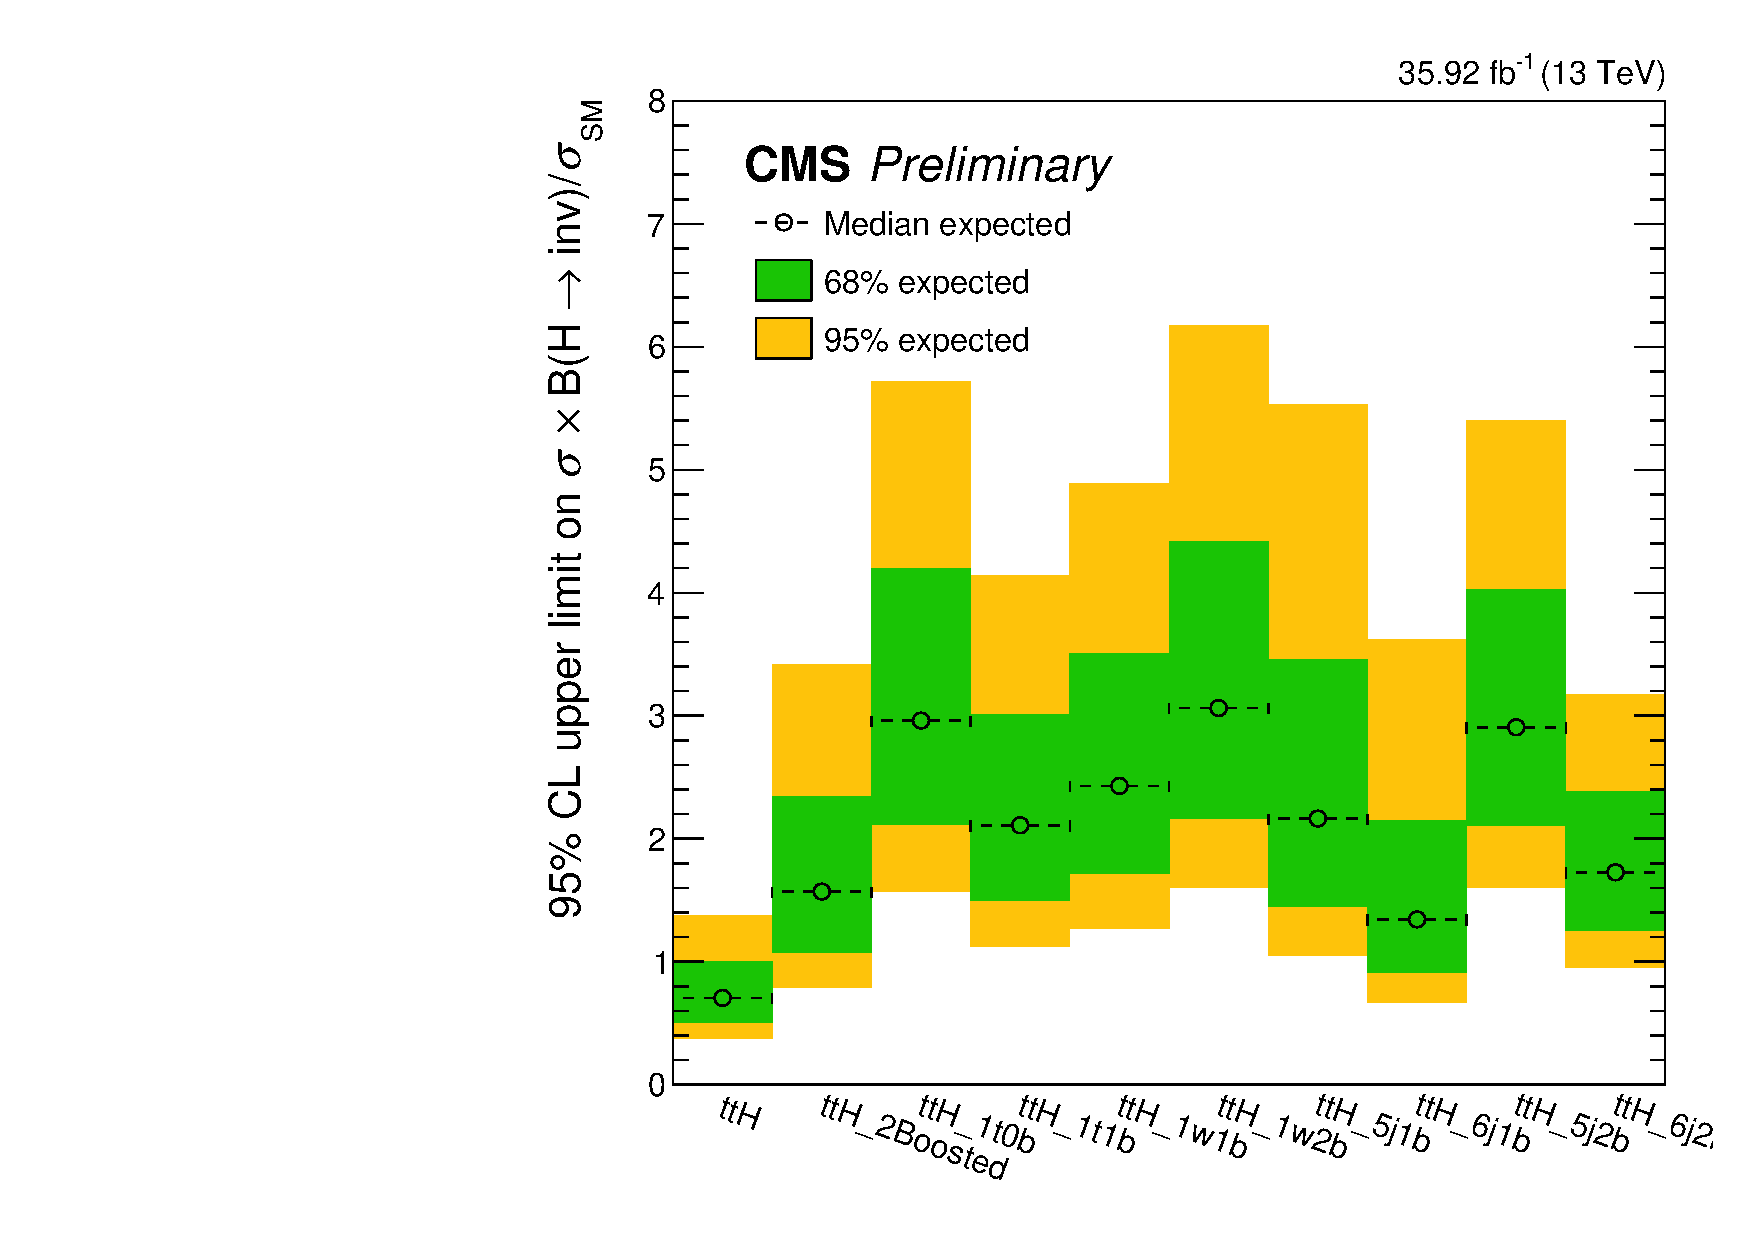
\includegraphics[width=\textwidth]{figures/limits/ttH/limit_2016_ttH_Scenario5.pdf}
        \caption{\ttH --- 2016}
    \end{subfigure}
    \hfill
    \begin{subfigure}[b]{0.45\textwidth}
        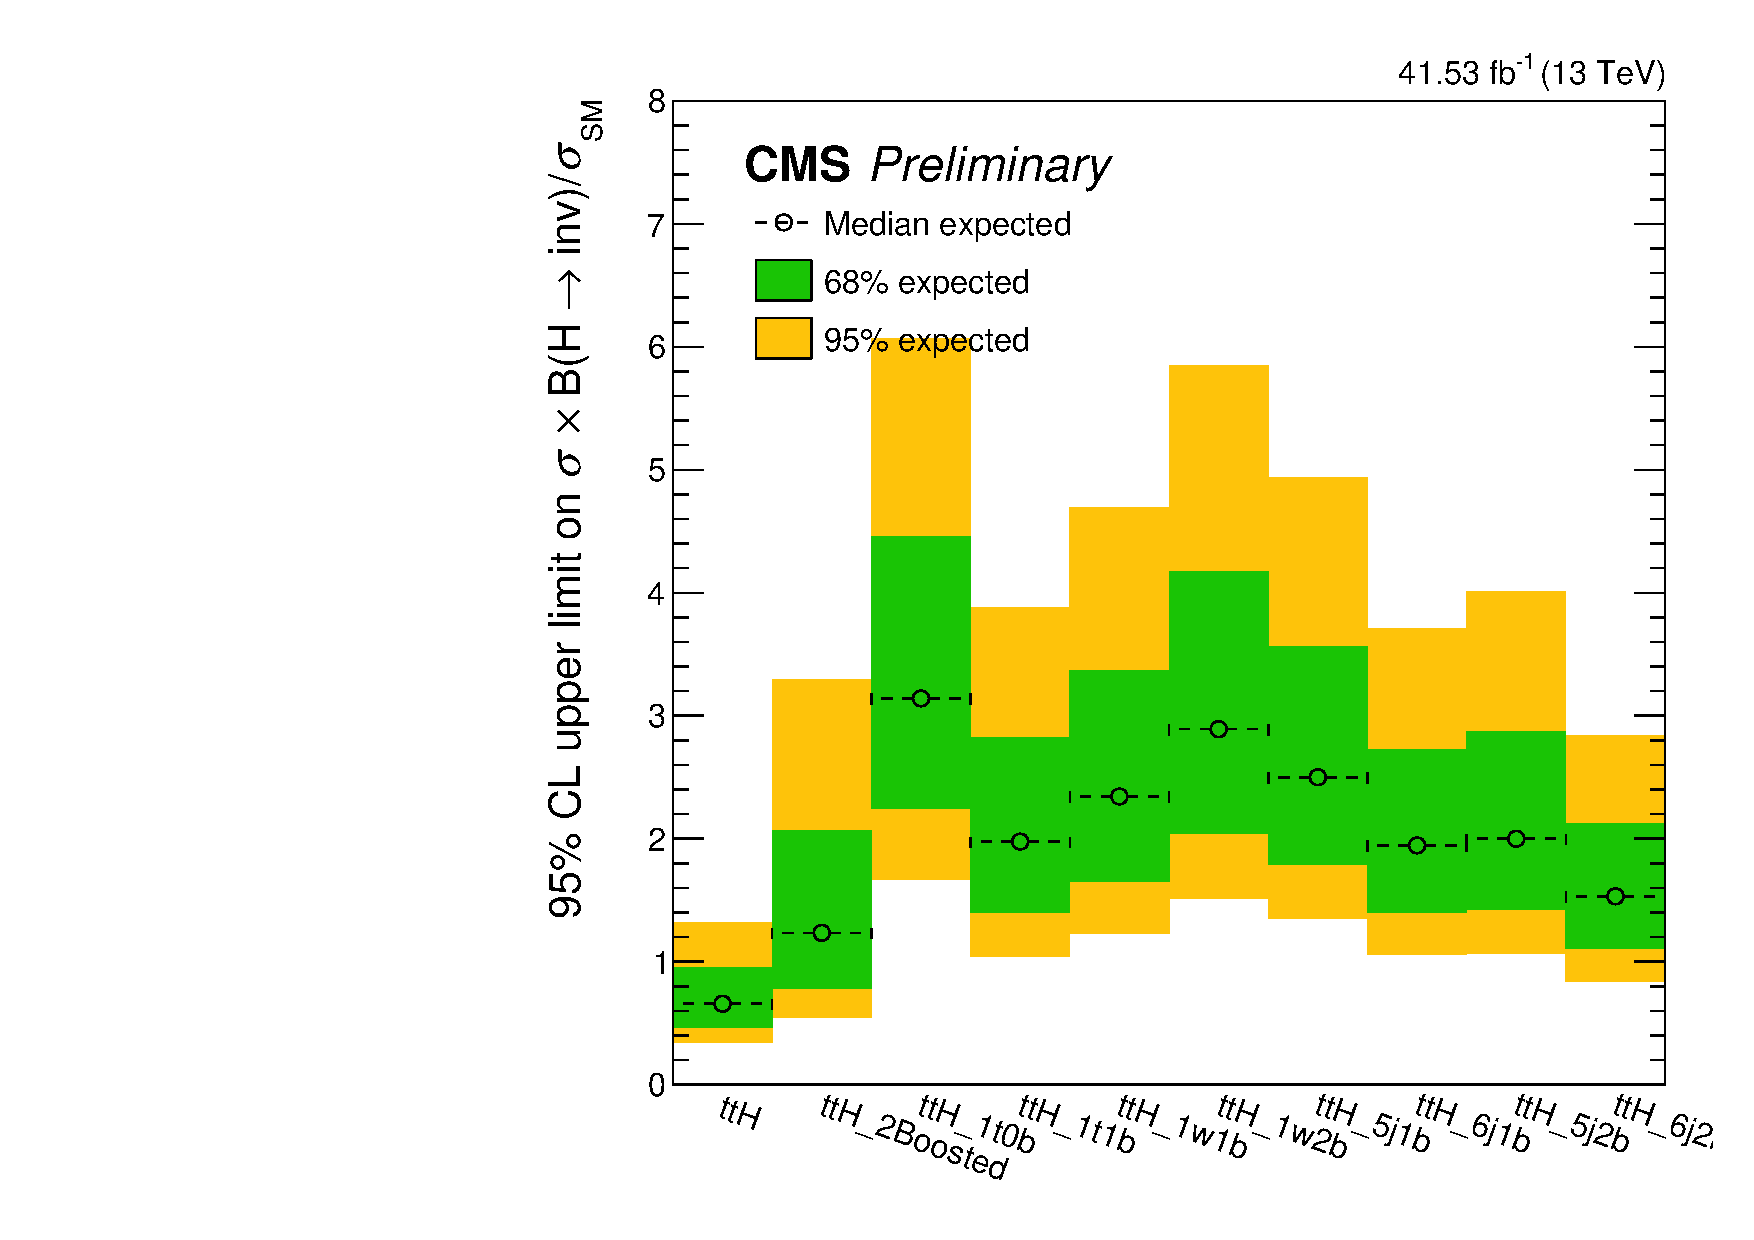
\includegraphics[width=\textwidth]{figures/limits/ttH/limit_2017_ttH_Scenario5.pdf}
        \caption{\ttH --- 2017}
    \end{subfigure}

    \begin{subfigure}[b]{0.45\textwidth}
        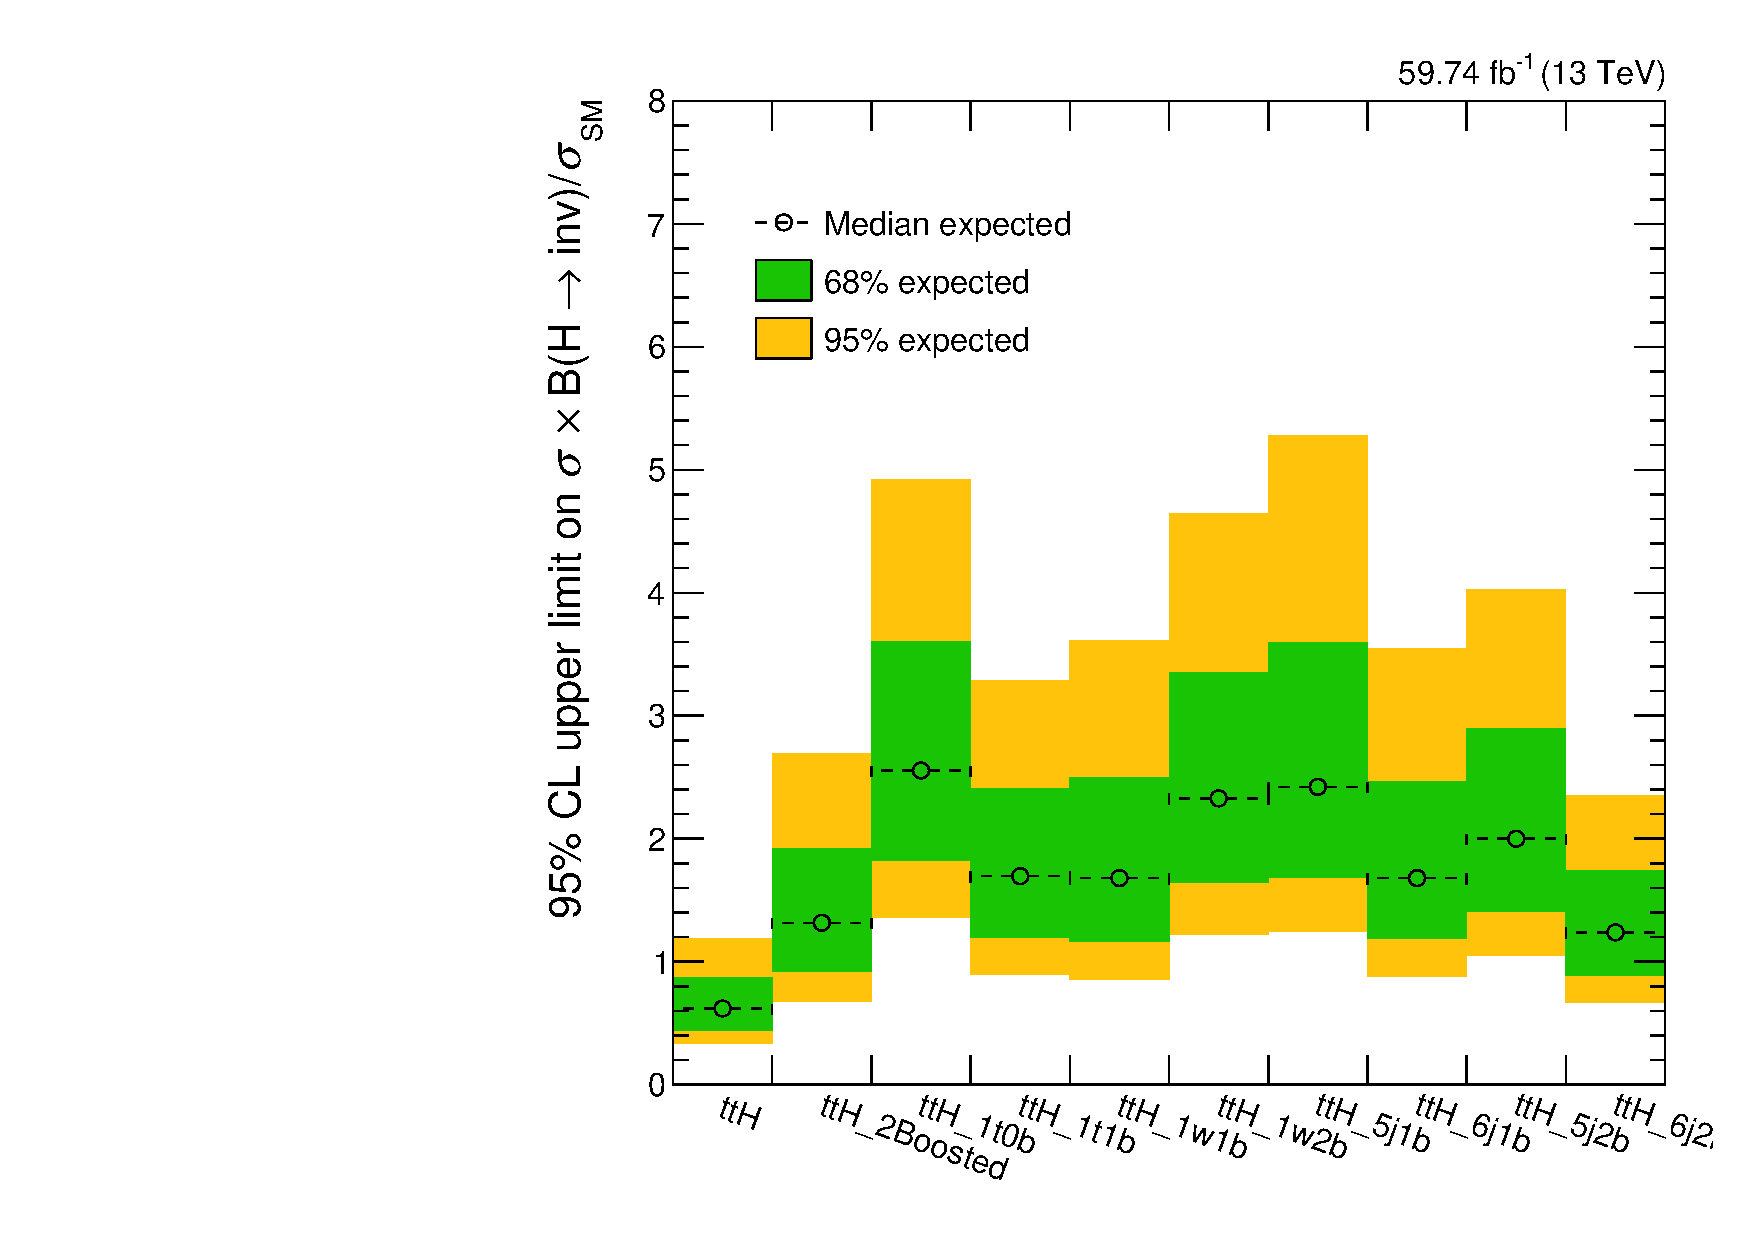
\includegraphics[width=\textwidth]{figures/limits/ttH/limit_2018_ttH_Scenario5.pdf}
        \caption{\ttH --- 2018}
    \end{subfigure}
    \hfill
    \begin{subfigure}[b]{0.45\textwidth}
        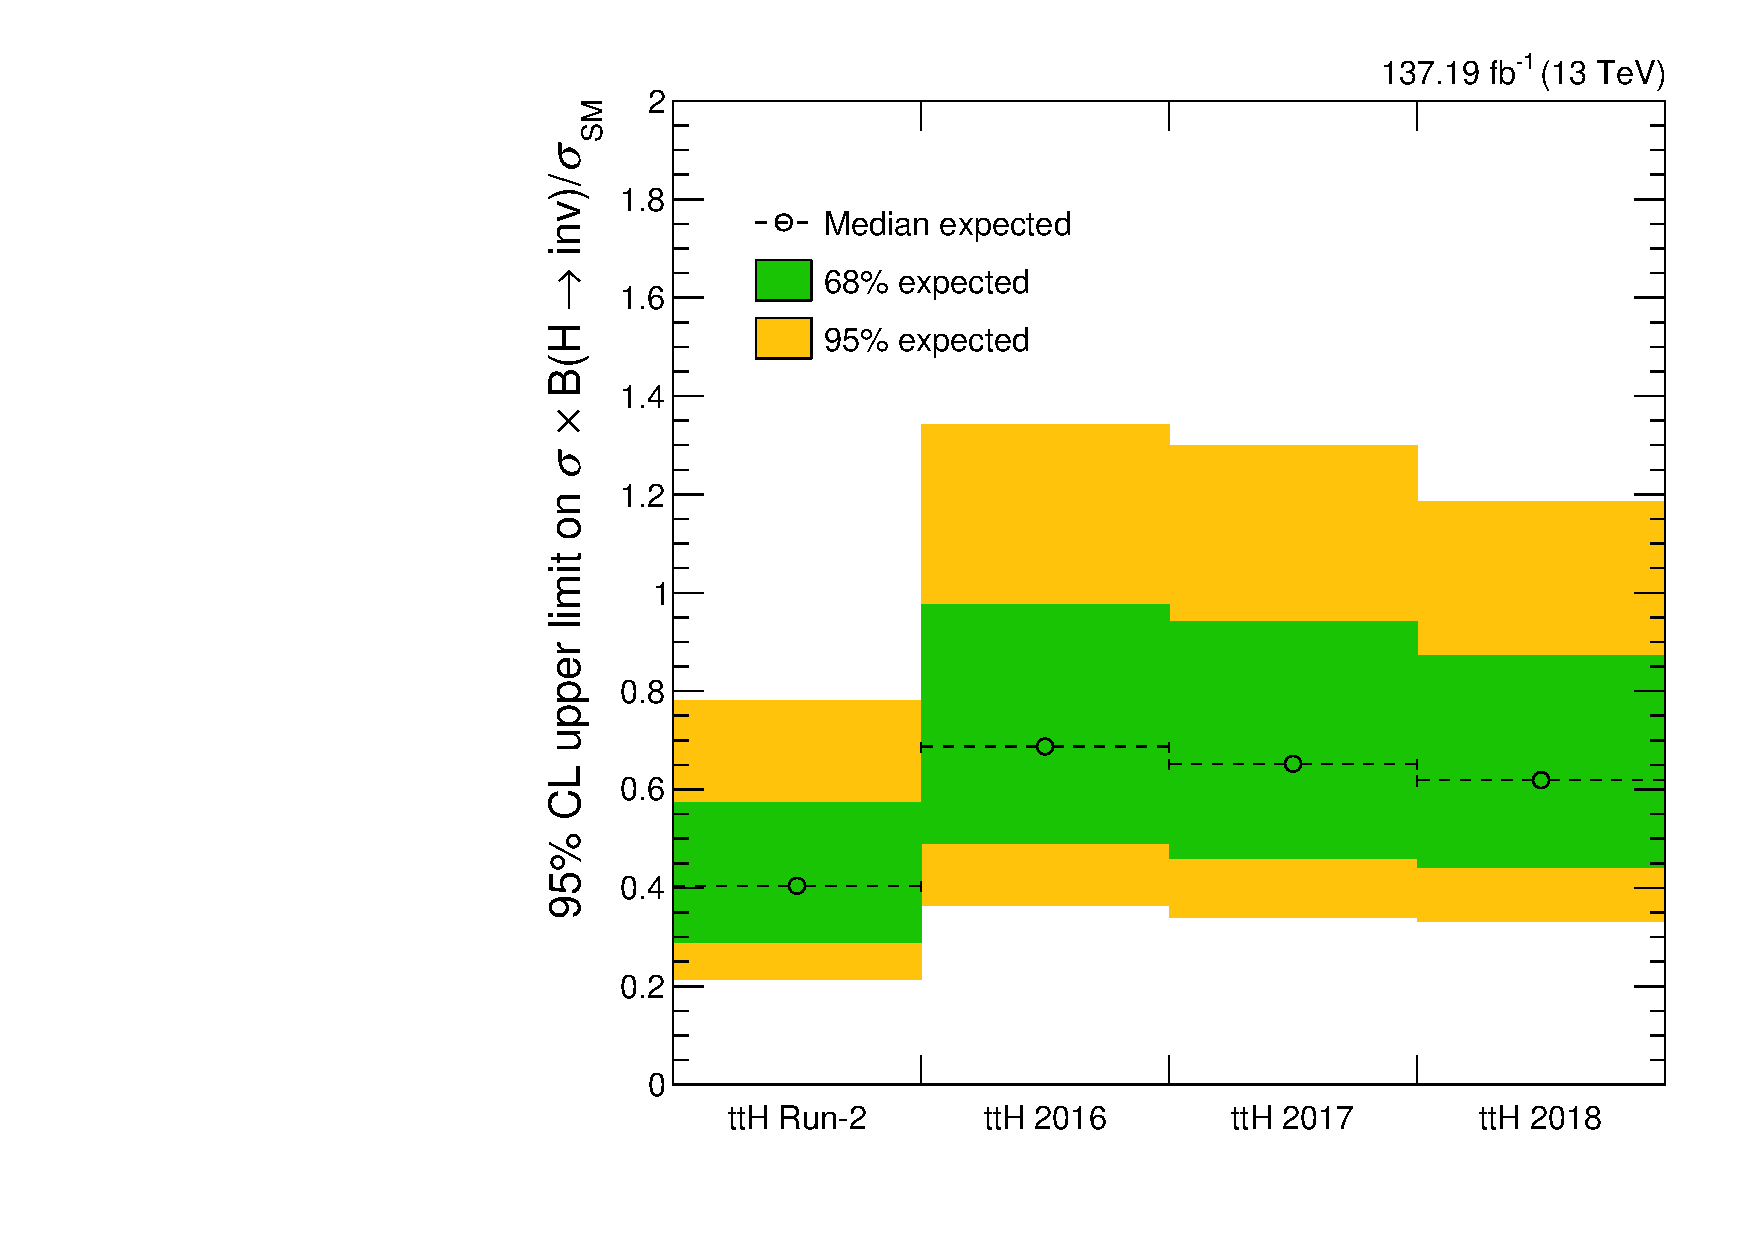
\includegraphics[width=\textwidth]{figures/limits/ttH/limit_Run2_ttH_Scenario5.pdf}
        \caption{\ttH --- Run-2}
    \end{subfigure}
    \caption[Expected 95\,\% CL upper limits on the Higgs boson to invisible state branching fraction in the \ttH category, for both the individual subcategories, and the combination of them, for each data-taking year in Run-2]{Expected 95\,\% CL upper limits on the Higgs boson to invisible state branching fraction in the \ttH category, for both the individual subcategories, and the combination of them, for each data-taking year in Run-2.}
    \label{fig:htoinv_limit_ttH}
\end{figure}


%=========================================================


\section{Analysis of the \texorpdfstring{\VH}{VH} mode}
\label{sec:htoinv_analysis_VH}

% Describe the specifics of the background estimation and fit for the VH subcategories, since they may differ for the other modes
% All CRs are used for non-multijet background estimation and predictions are fully granular
% Not sure how we'll do QCD estimation for VH. Potentially same methods as ttH and ggF but using different sidebands

Fig.~\ref{fig:htoinv_limit_VH} showcases the median expected limit on $\BRof{\higgstoinv}$ with 1$\sigma$ and 2$\sigma$ bounds for the \VH category and its subcategories.

\begin{figure}[htbp]
    \centering
    \begin{subfigure}[b]{0.45\textwidth}
        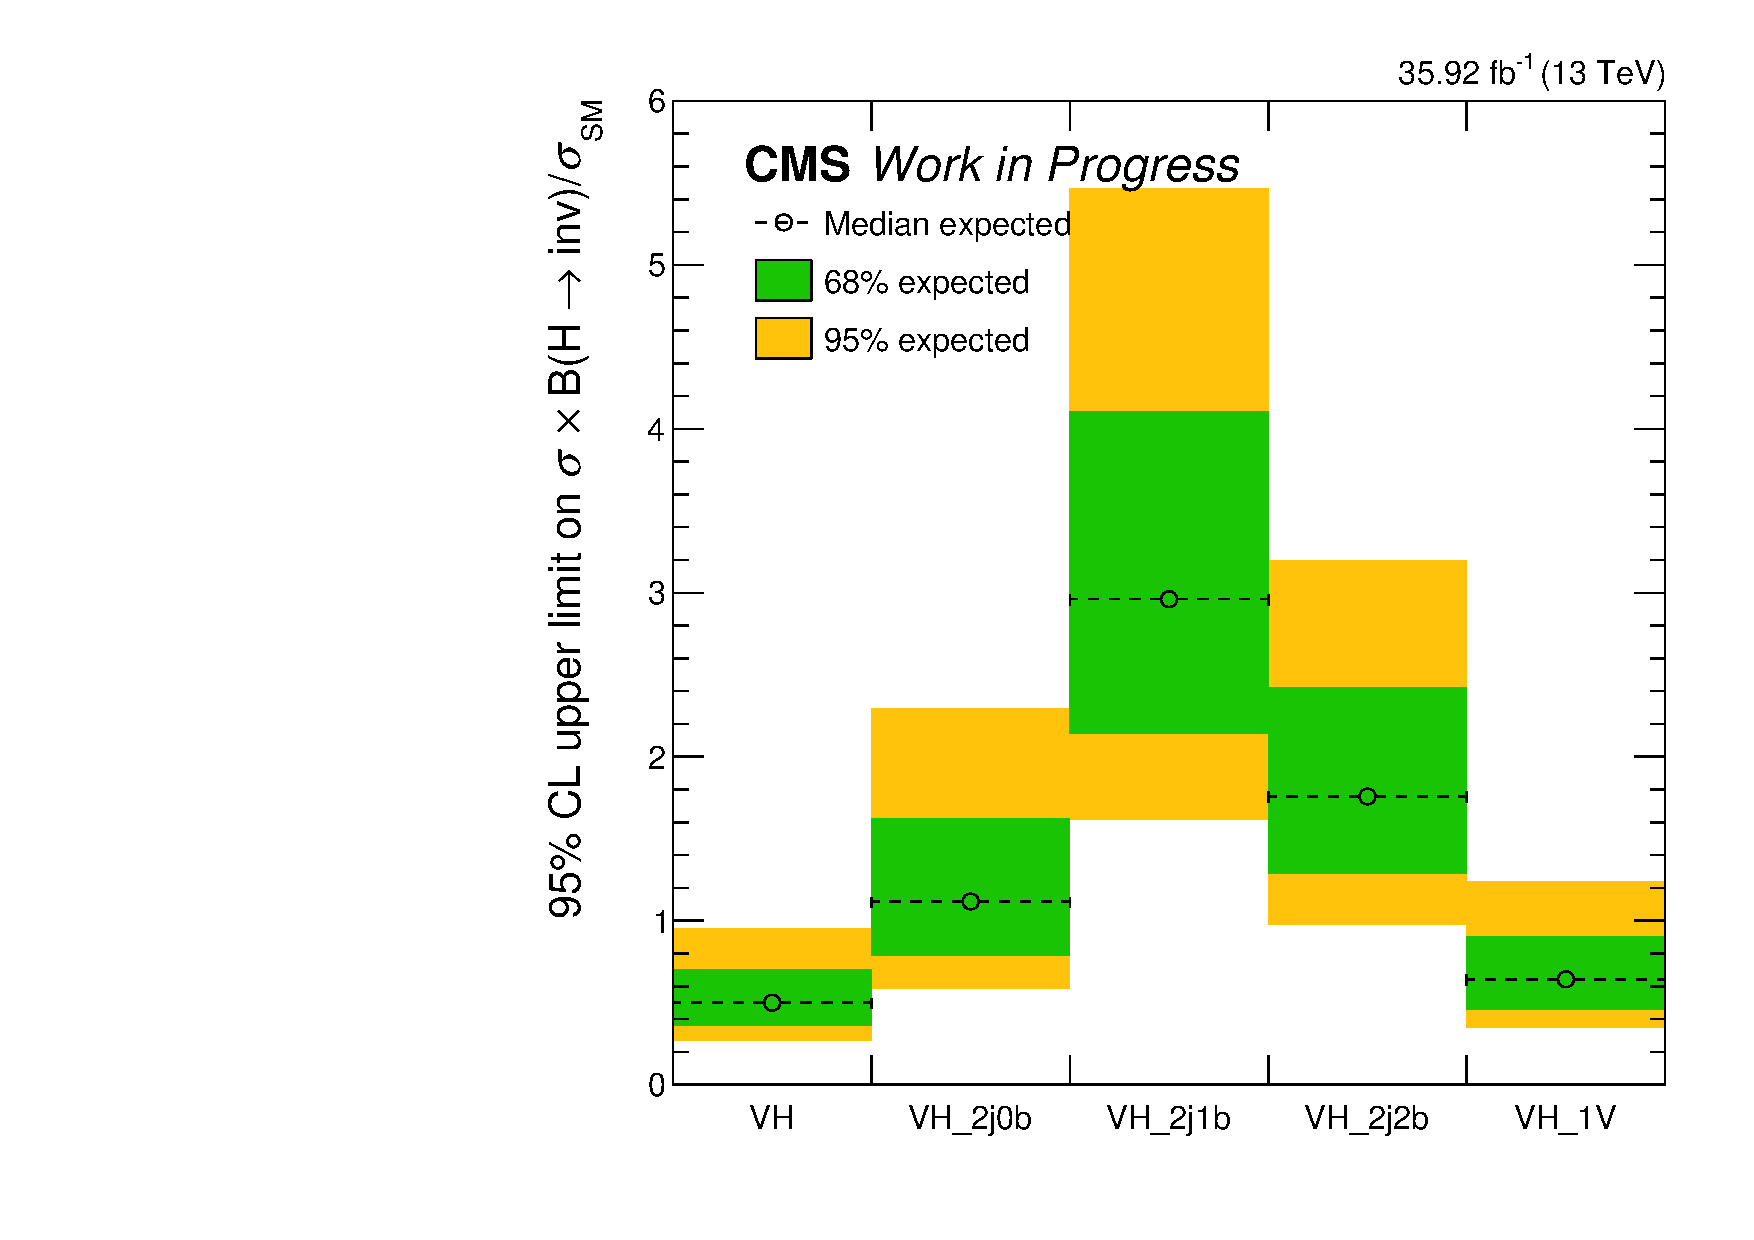
\includegraphics[width=\textwidth]{figures/limits/VH/limit_2016_VH_Scenario5.pdf}
        \caption{\VH --- 2016}
    \end{subfigure}
    \hfill
    \begin{subfigure}[b]{0.45\textwidth}
        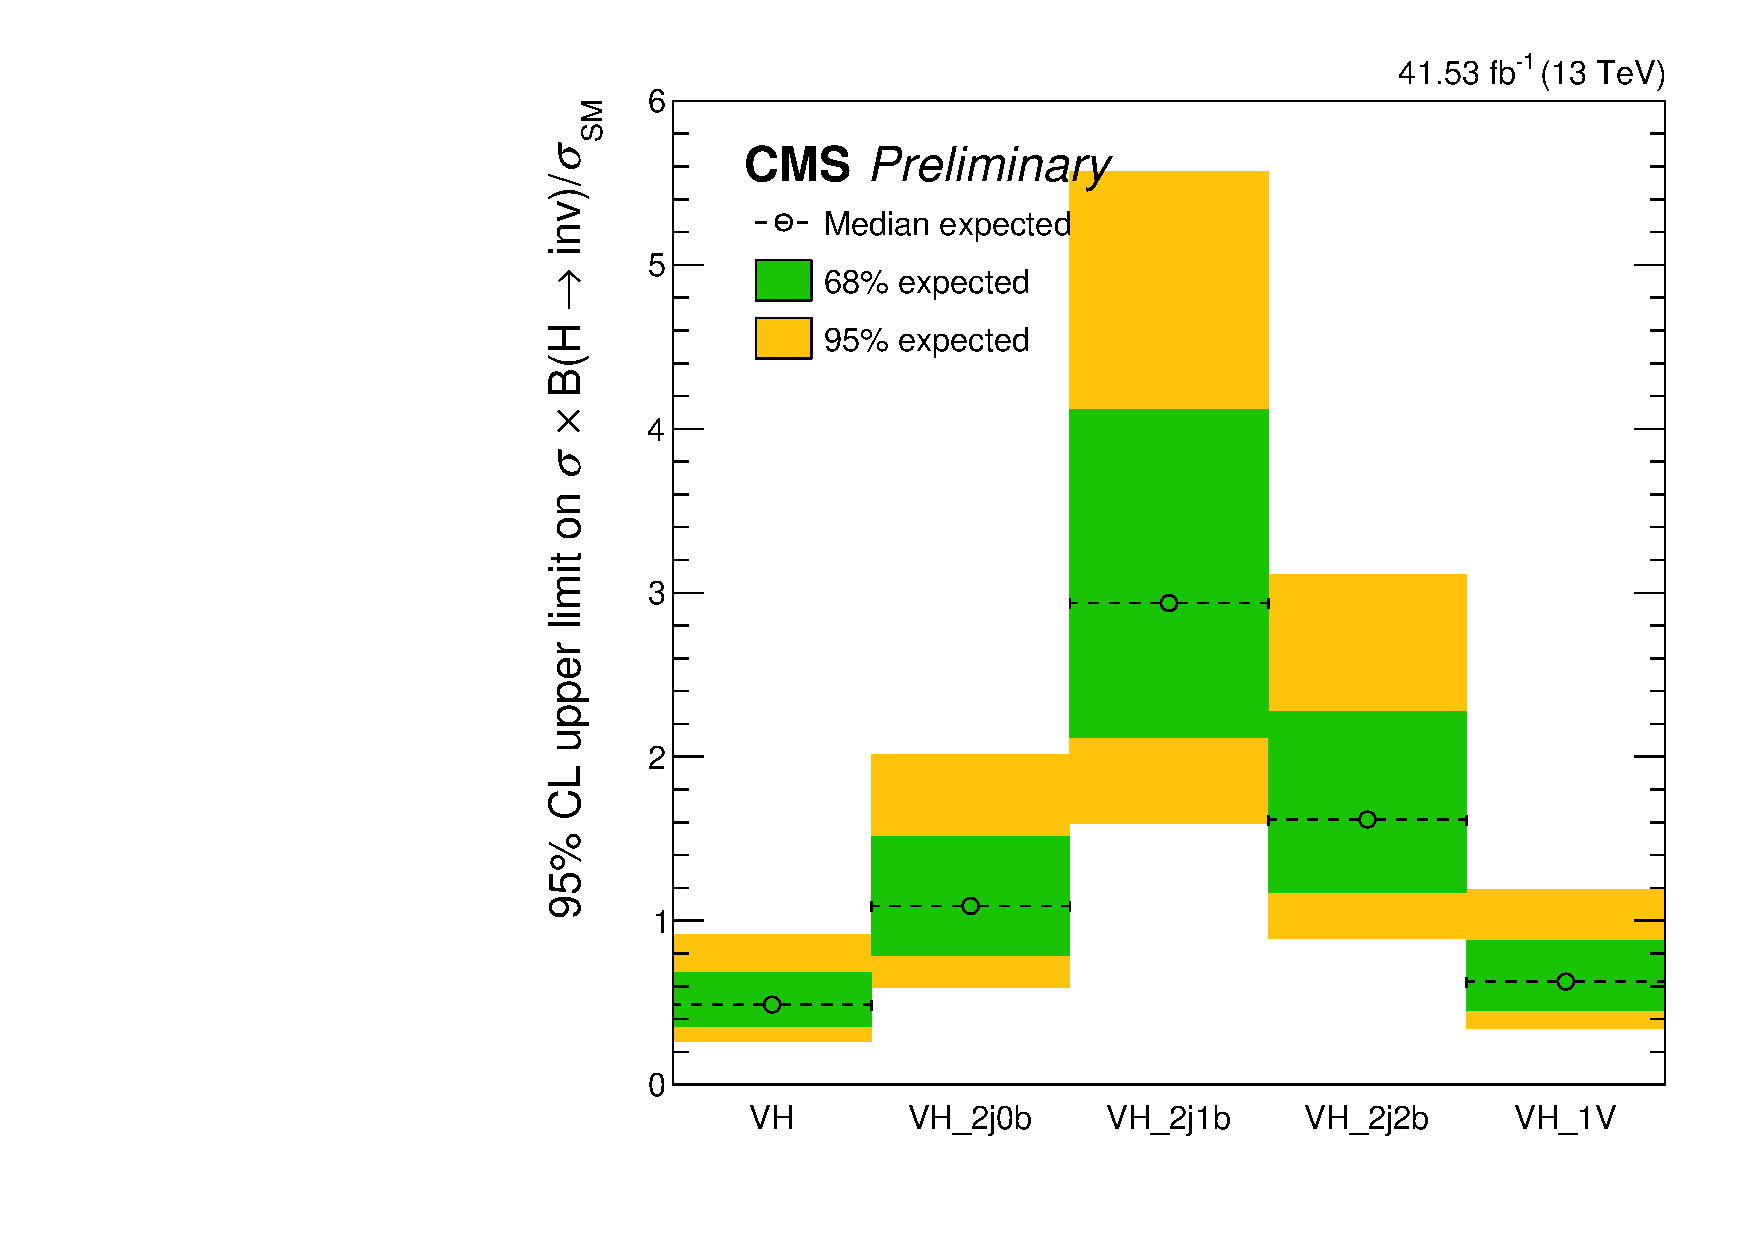
\includegraphics[width=\textwidth]{figures/limits/VH/limit_2017_VH_Scenario5.pdf}
        \caption{\VH --- 2017}
    \end{subfigure}

    \begin{subfigure}[b]{0.45\textwidth}
        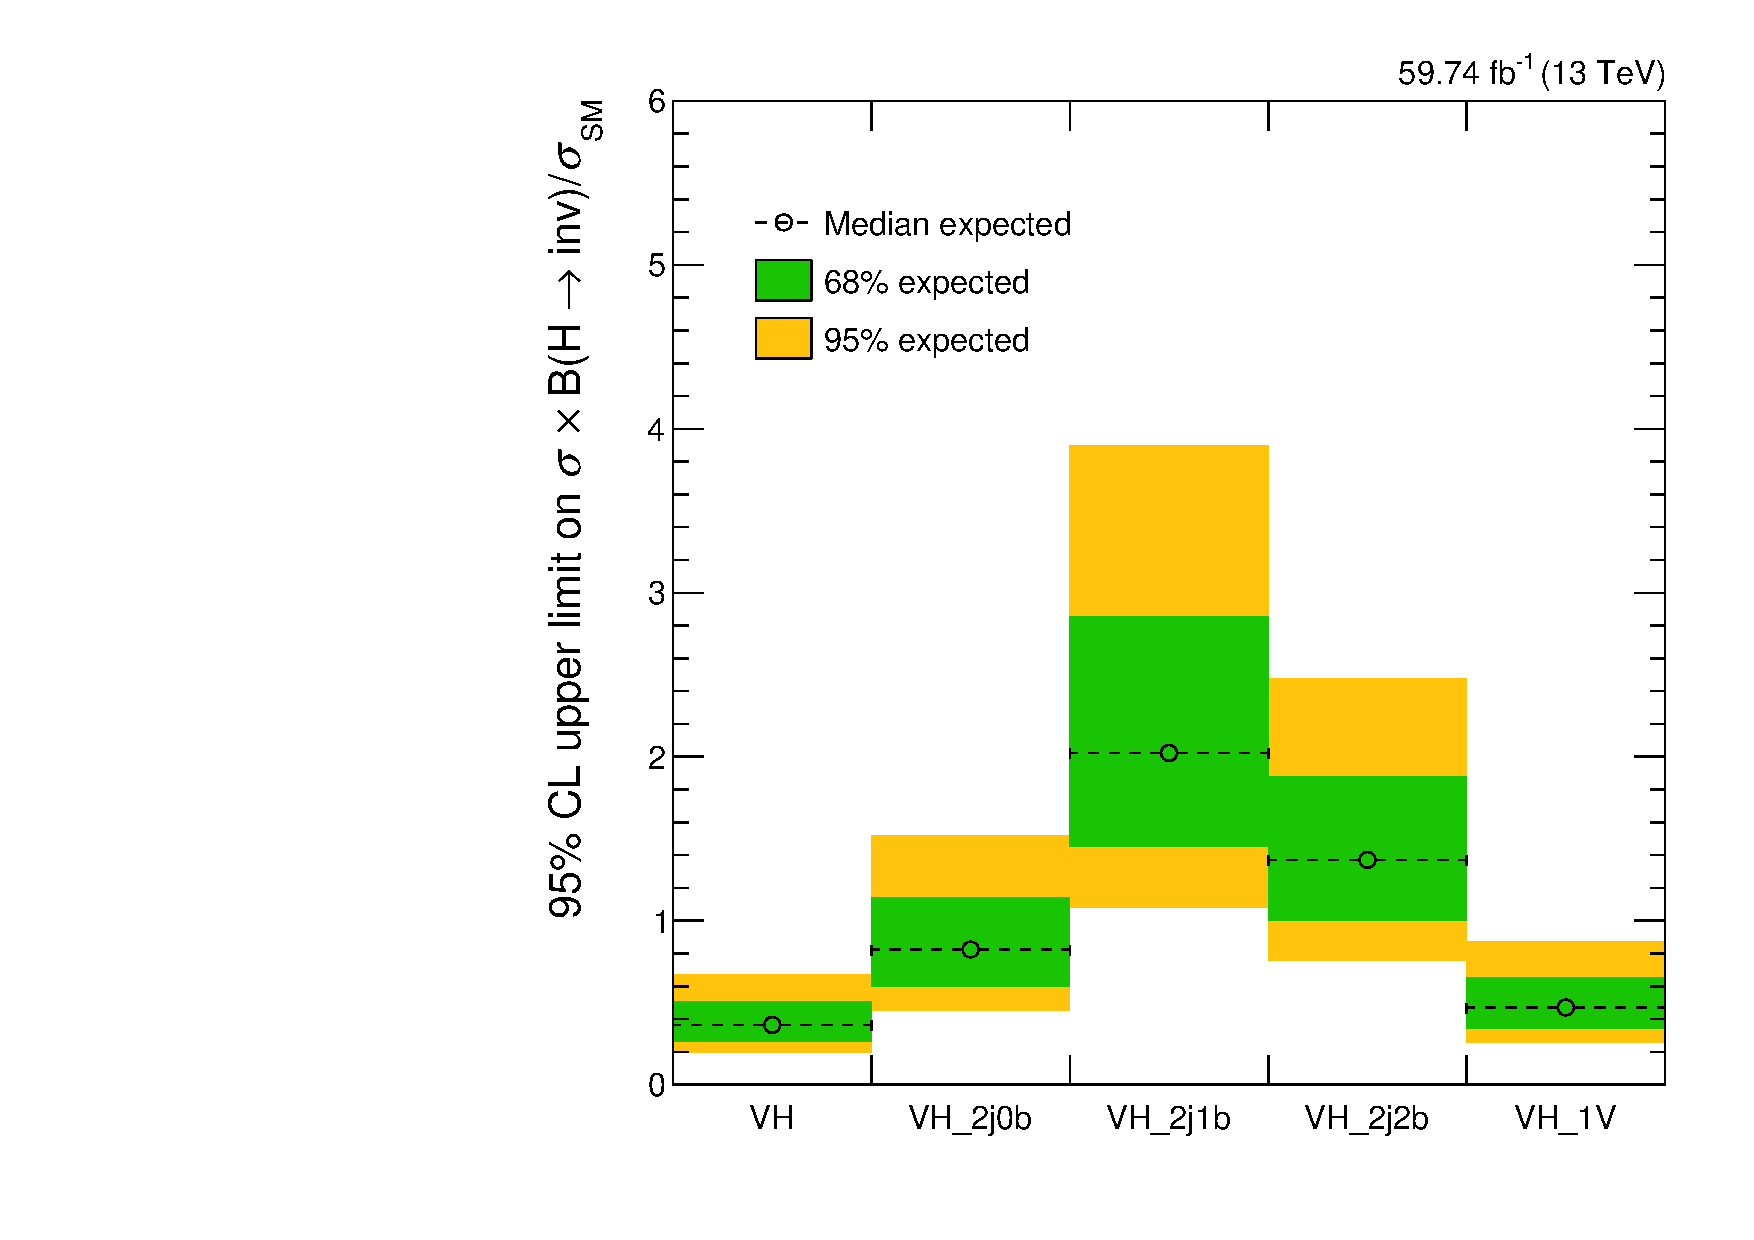
\includegraphics[width=\textwidth]{figures/limits/VH/limit_2018_VH_Scenario5.pdf}
        \caption{\VH --- 2018}
    \end{subfigure}
    \hfill
    \begin{subfigure}[b]{0.45\textwidth}
        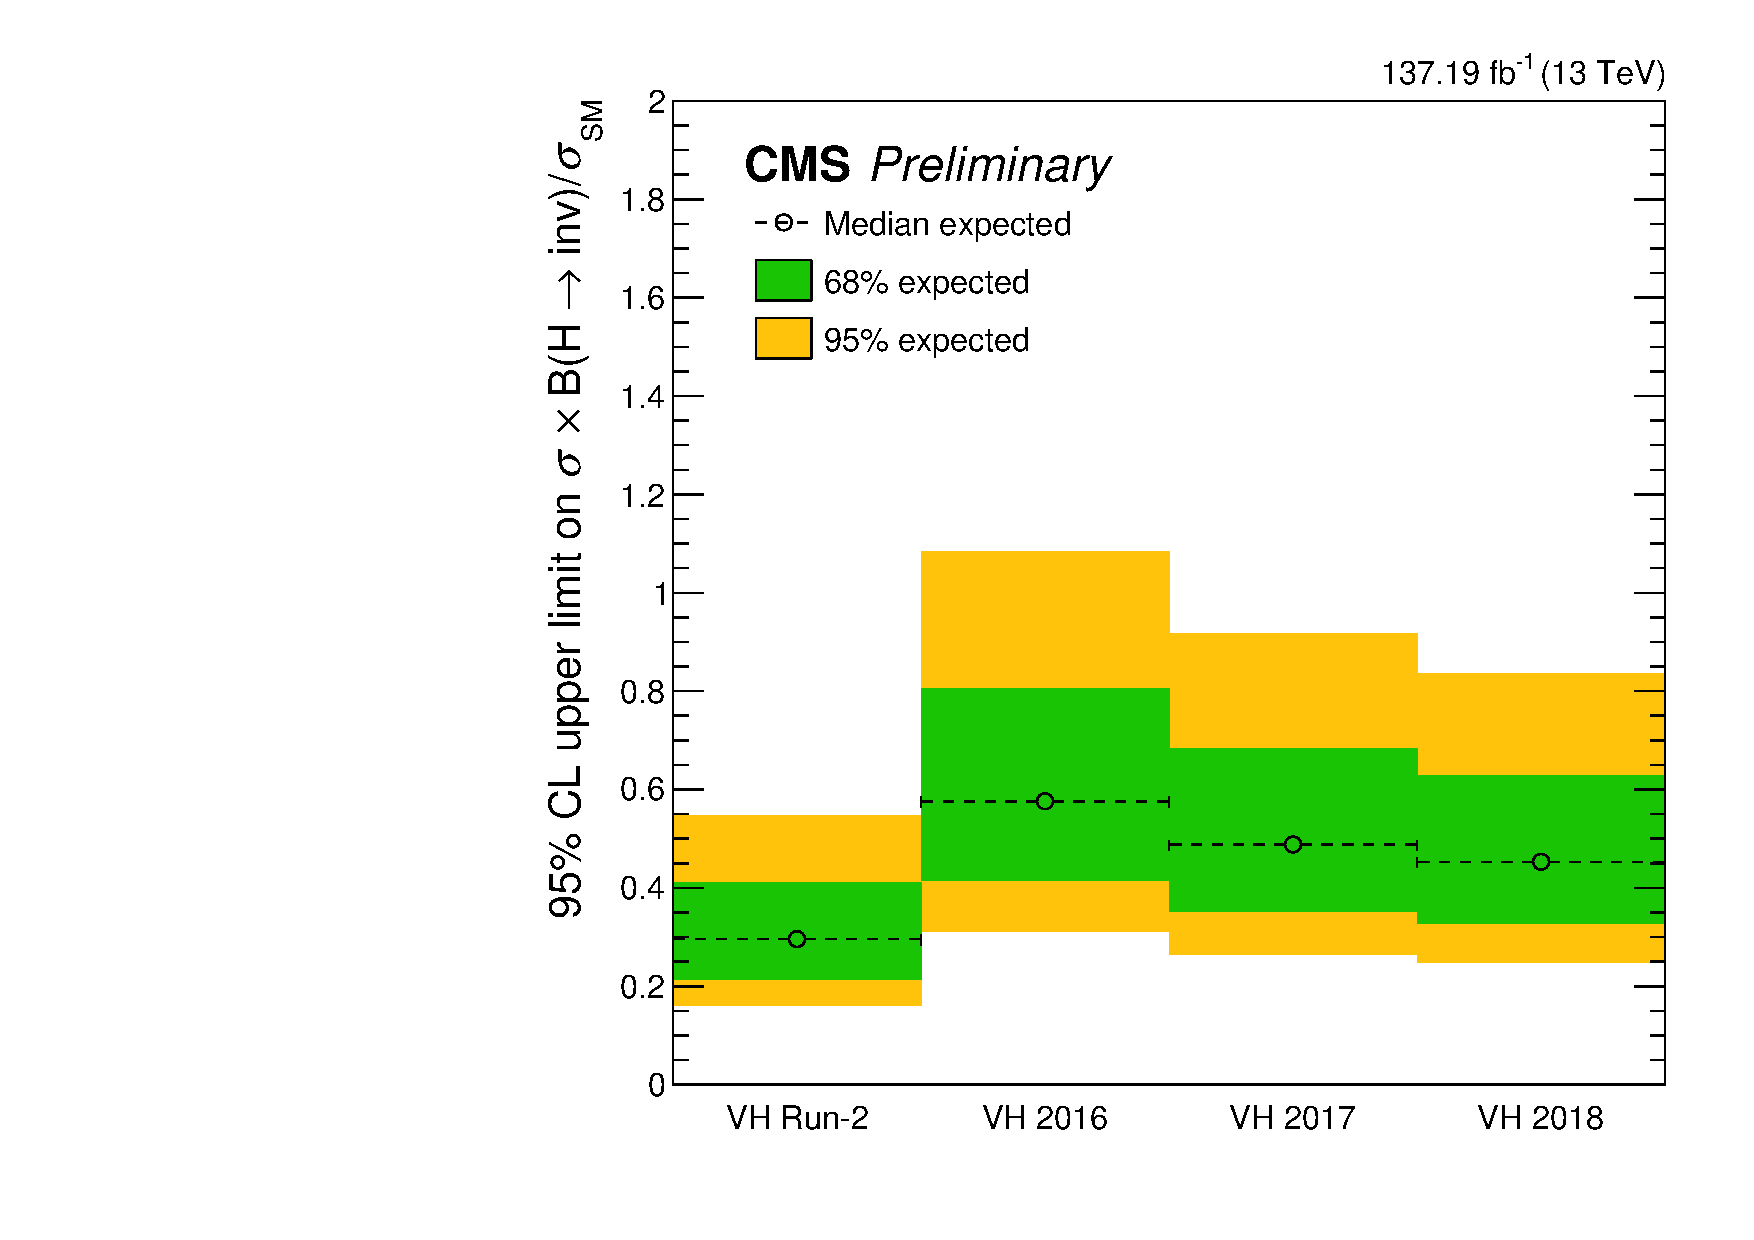
\includegraphics[width=\textwidth]{figures/limits/VH/limit_Run2_VH_Scenario5.pdf}
        \caption{\VH --- Run-2}
    \end{subfigure}
    \caption[Expected 95\,\% CL upper limits on the Higgs boson to invisible state branching fraction in the \VH category, for both the individual subcategories, and the combination of them, for each data-taking year in Run-2]{Expected 95\,\% CL upper limits on the Higgs boson to invisible state branching fraction in the \VH category, for both the individual subcategories, and the combination of them, for each data-taking year in Run-2.}
    \label{fig:htoinv_limit_VH}
\end{figure}


%=========================================================


\section{Analysis of the \texorpdfstring{\ggH}{ggH} mode}
\label{sec:htoinv_analysis_ggF}

% Describe the specifics of the background estimation and fit for ggF subcategories, since they may differ for the other modes
% Like VH, non-multijet background estimation is done with all CRs and fully granular
% Like ttH, QCD background estimation is done with sideband 0 to derive category fraction, then sideband 2 for MET fraction and transfer factor

Fig.~\ref{fig:htoinv_limit_ggF} showcases the median expected limit on $\BRof{\higgstoinv}$ with 1$\sigma$ and 2$\sigma$ bounds for the \ggH category and its subcategories.

\begin{figure}[htbp]
    \centering
    \begin{subfigure}[b]{0.45\textwidth}
        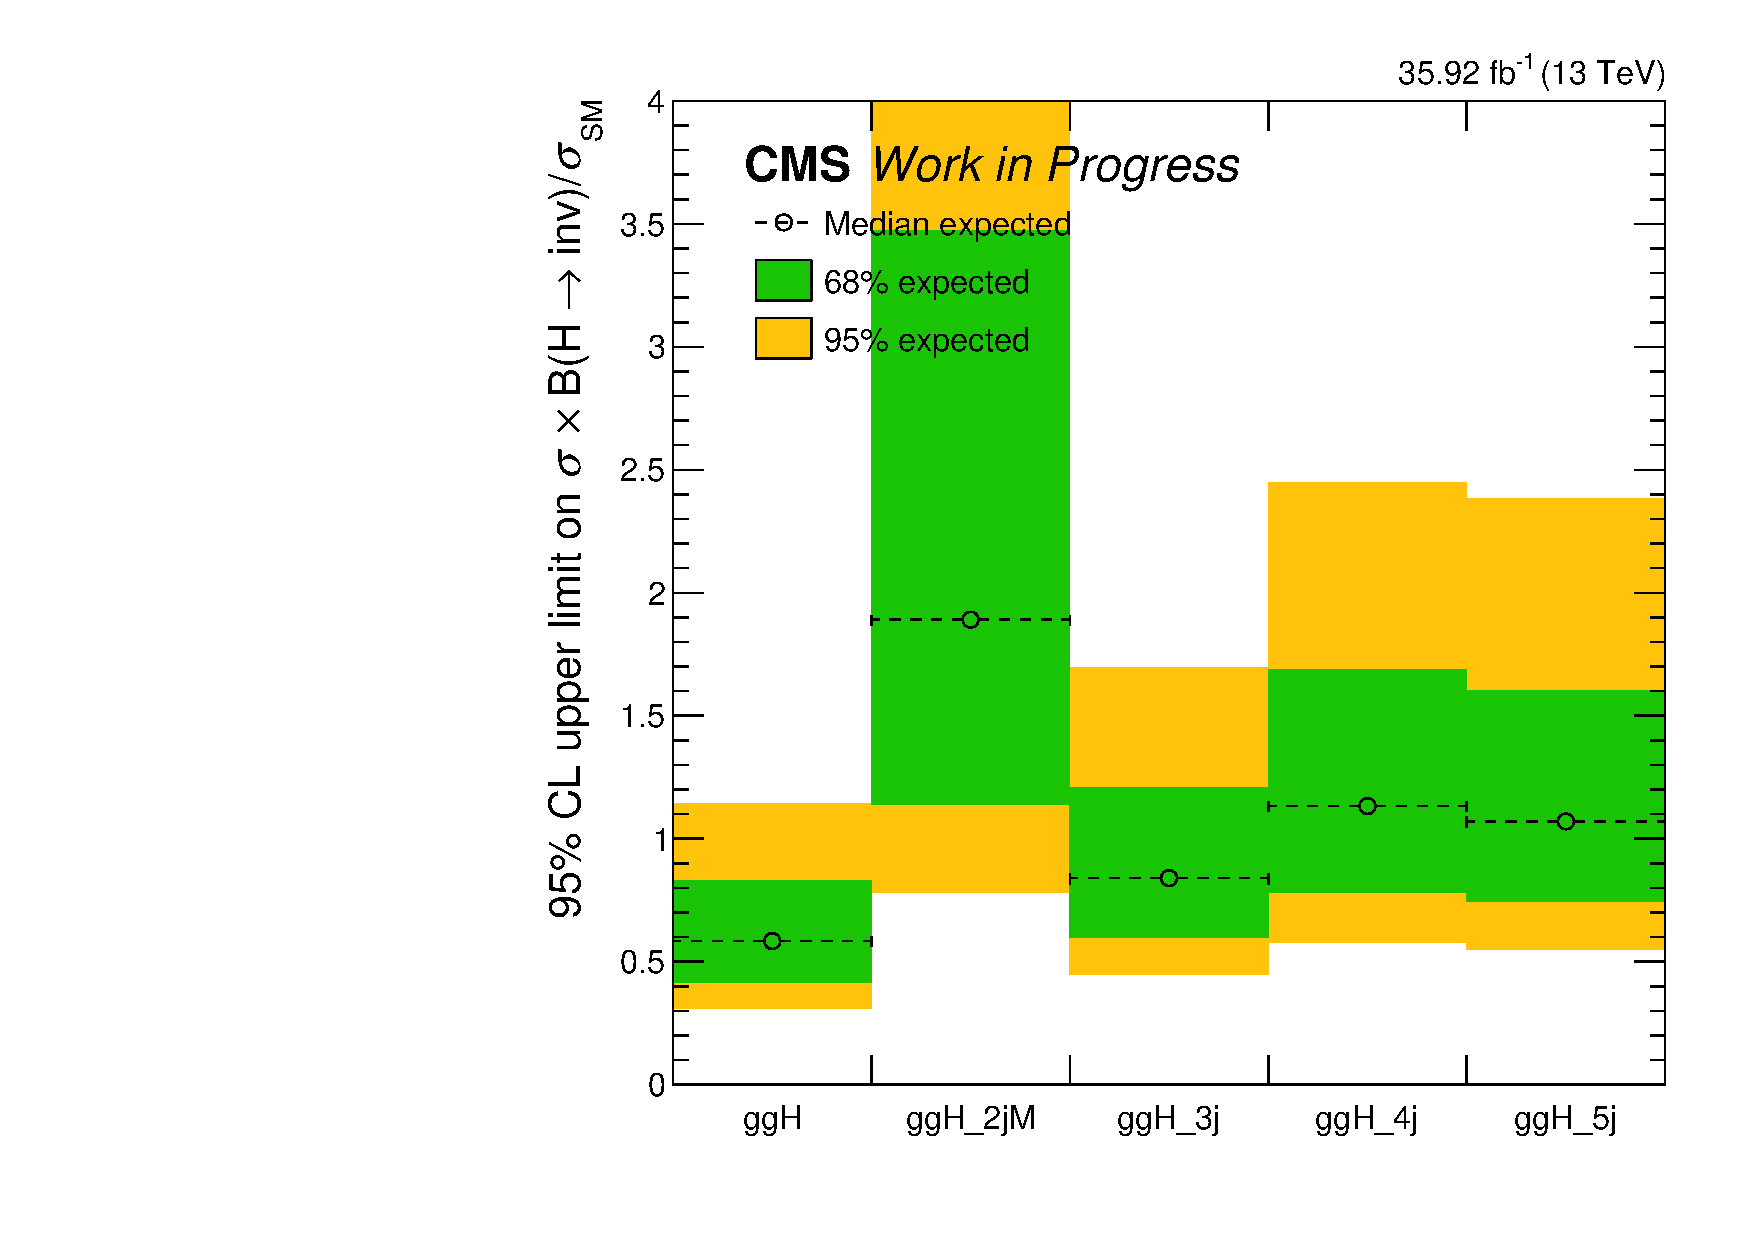
\includegraphics[width=\textwidth]{figures/limits/ggF/limit_2016_ggF_Scenario5.pdf}
        \caption{\ggH --- 2016}
    \end{subfigure}
    \hfill
    \begin{subfigure}[b]{0.45\textwidth}
        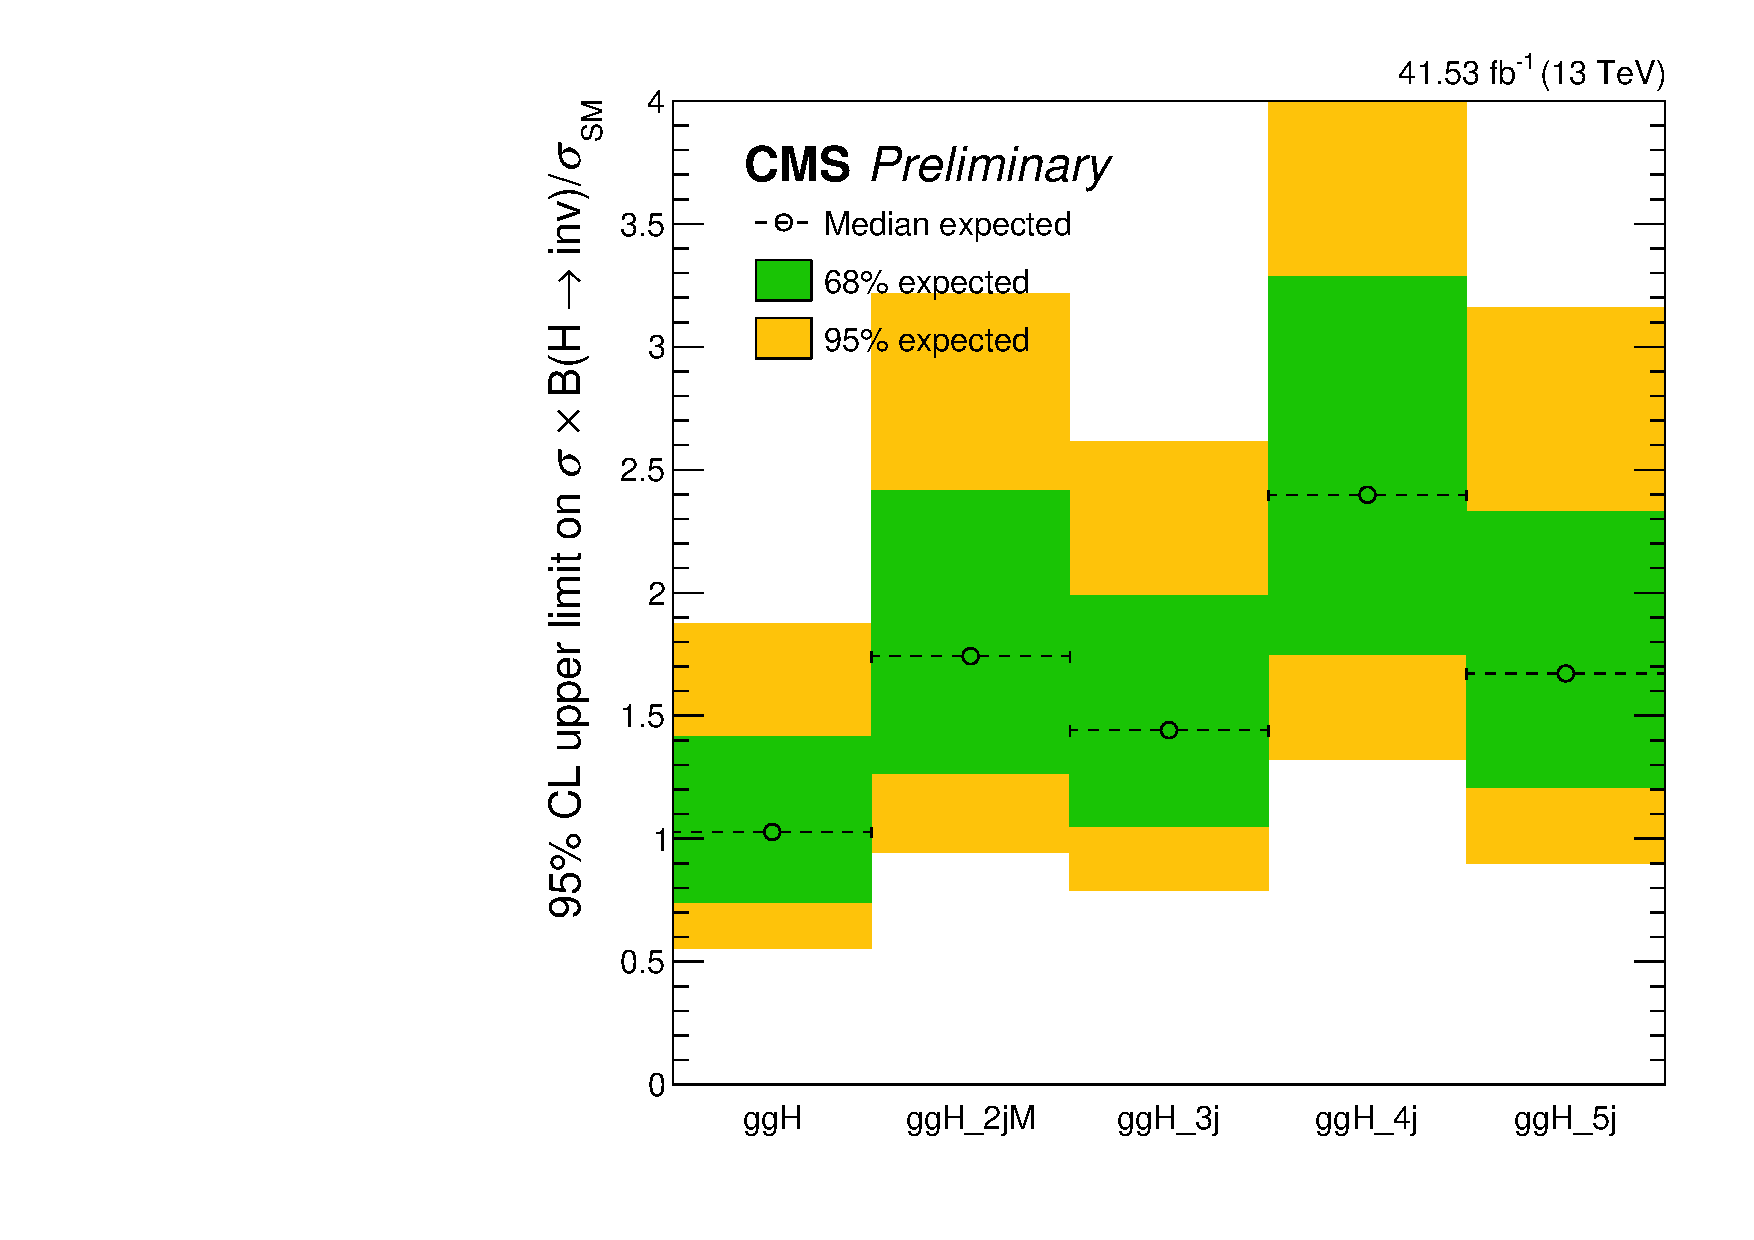
\includegraphics[width=\textwidth]{figures/limits/ggF/limit_2017_ggF_Scenario5.pdf}
        \caption{\ggH --- 2017}
    \end{subfigure}

    \begin{subfigure}[b]{0.45\textwidth}
        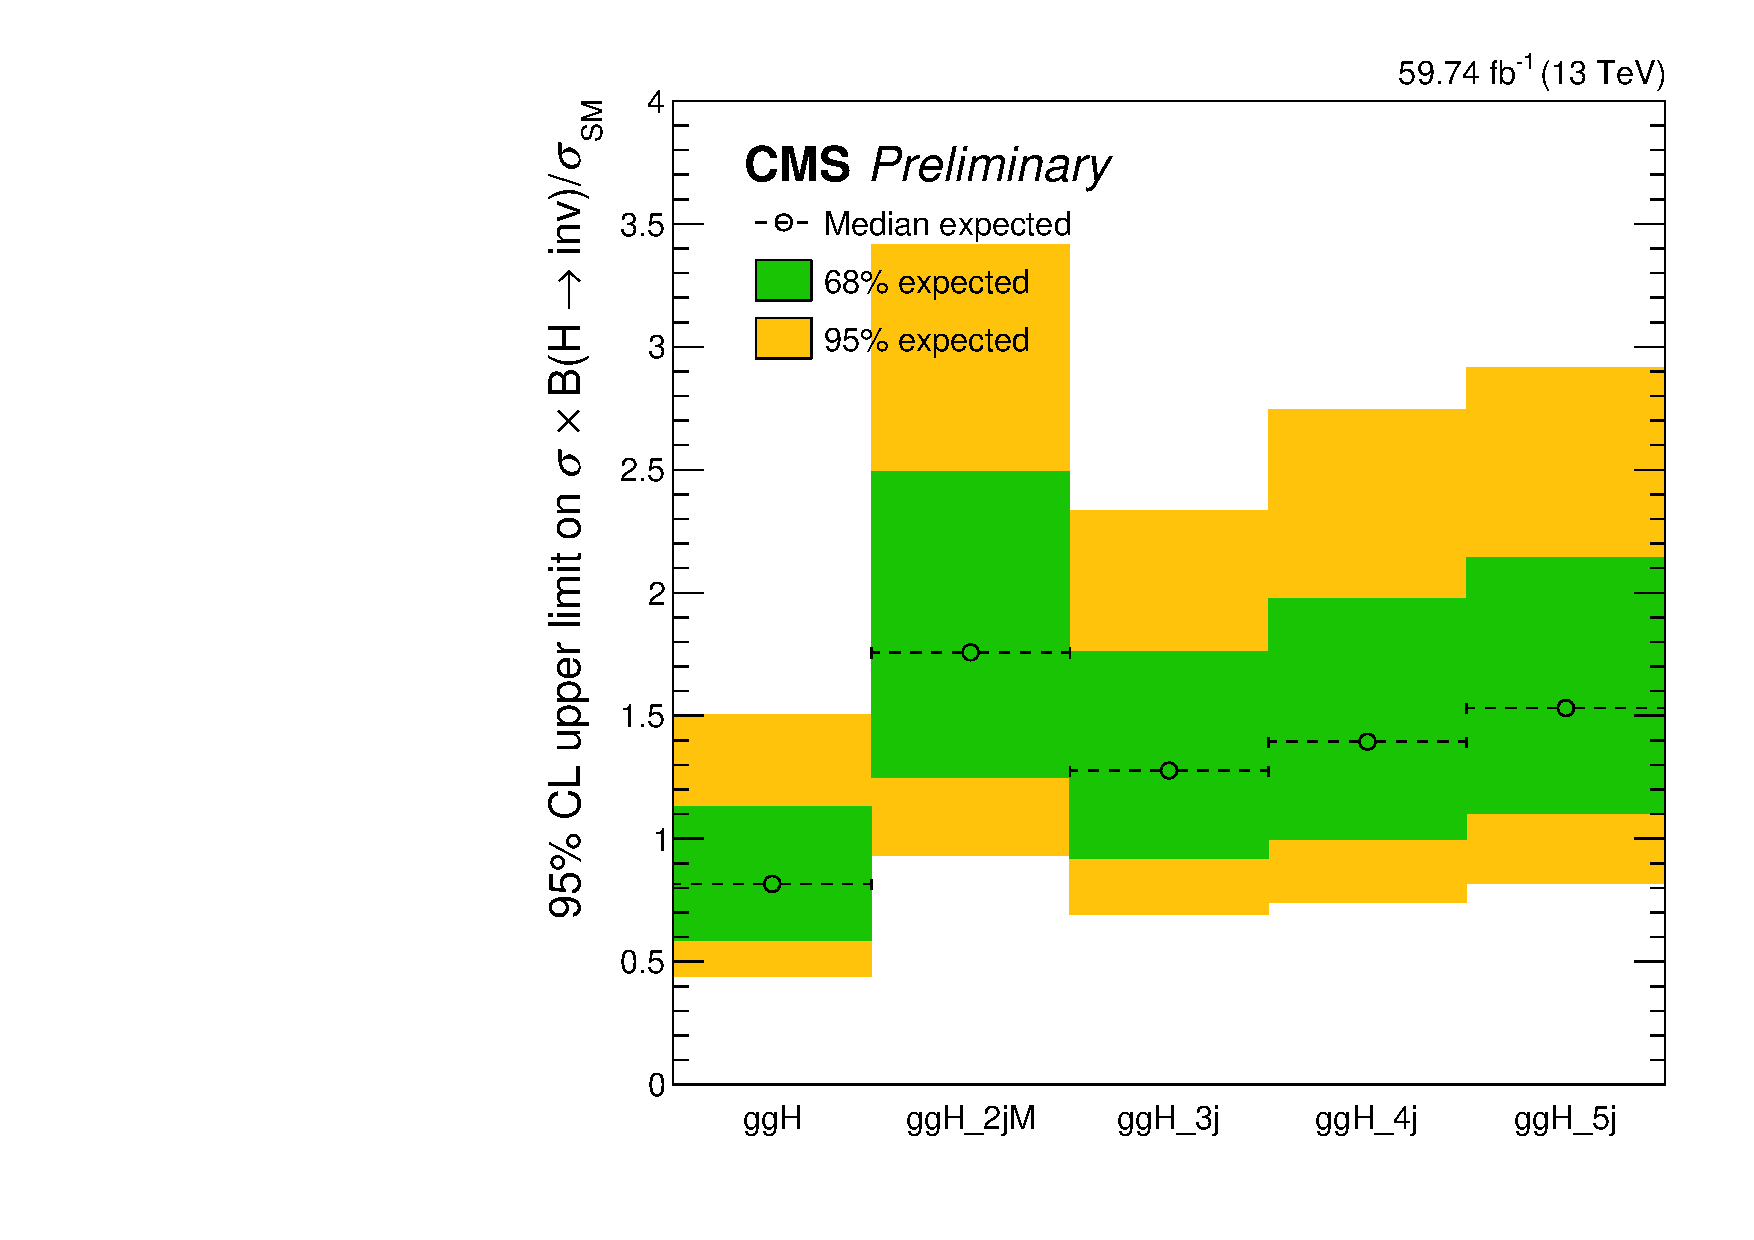
\includegraphics[width=\textwidth]{figures/limits/ggF/limit_2018_ggF_Scenario5.pdf}
        \caption{\ggH --- 2018}
    \end{subfigure}
    \hfill
    \begin{subfigure}[b]{0.45\textwidth}
        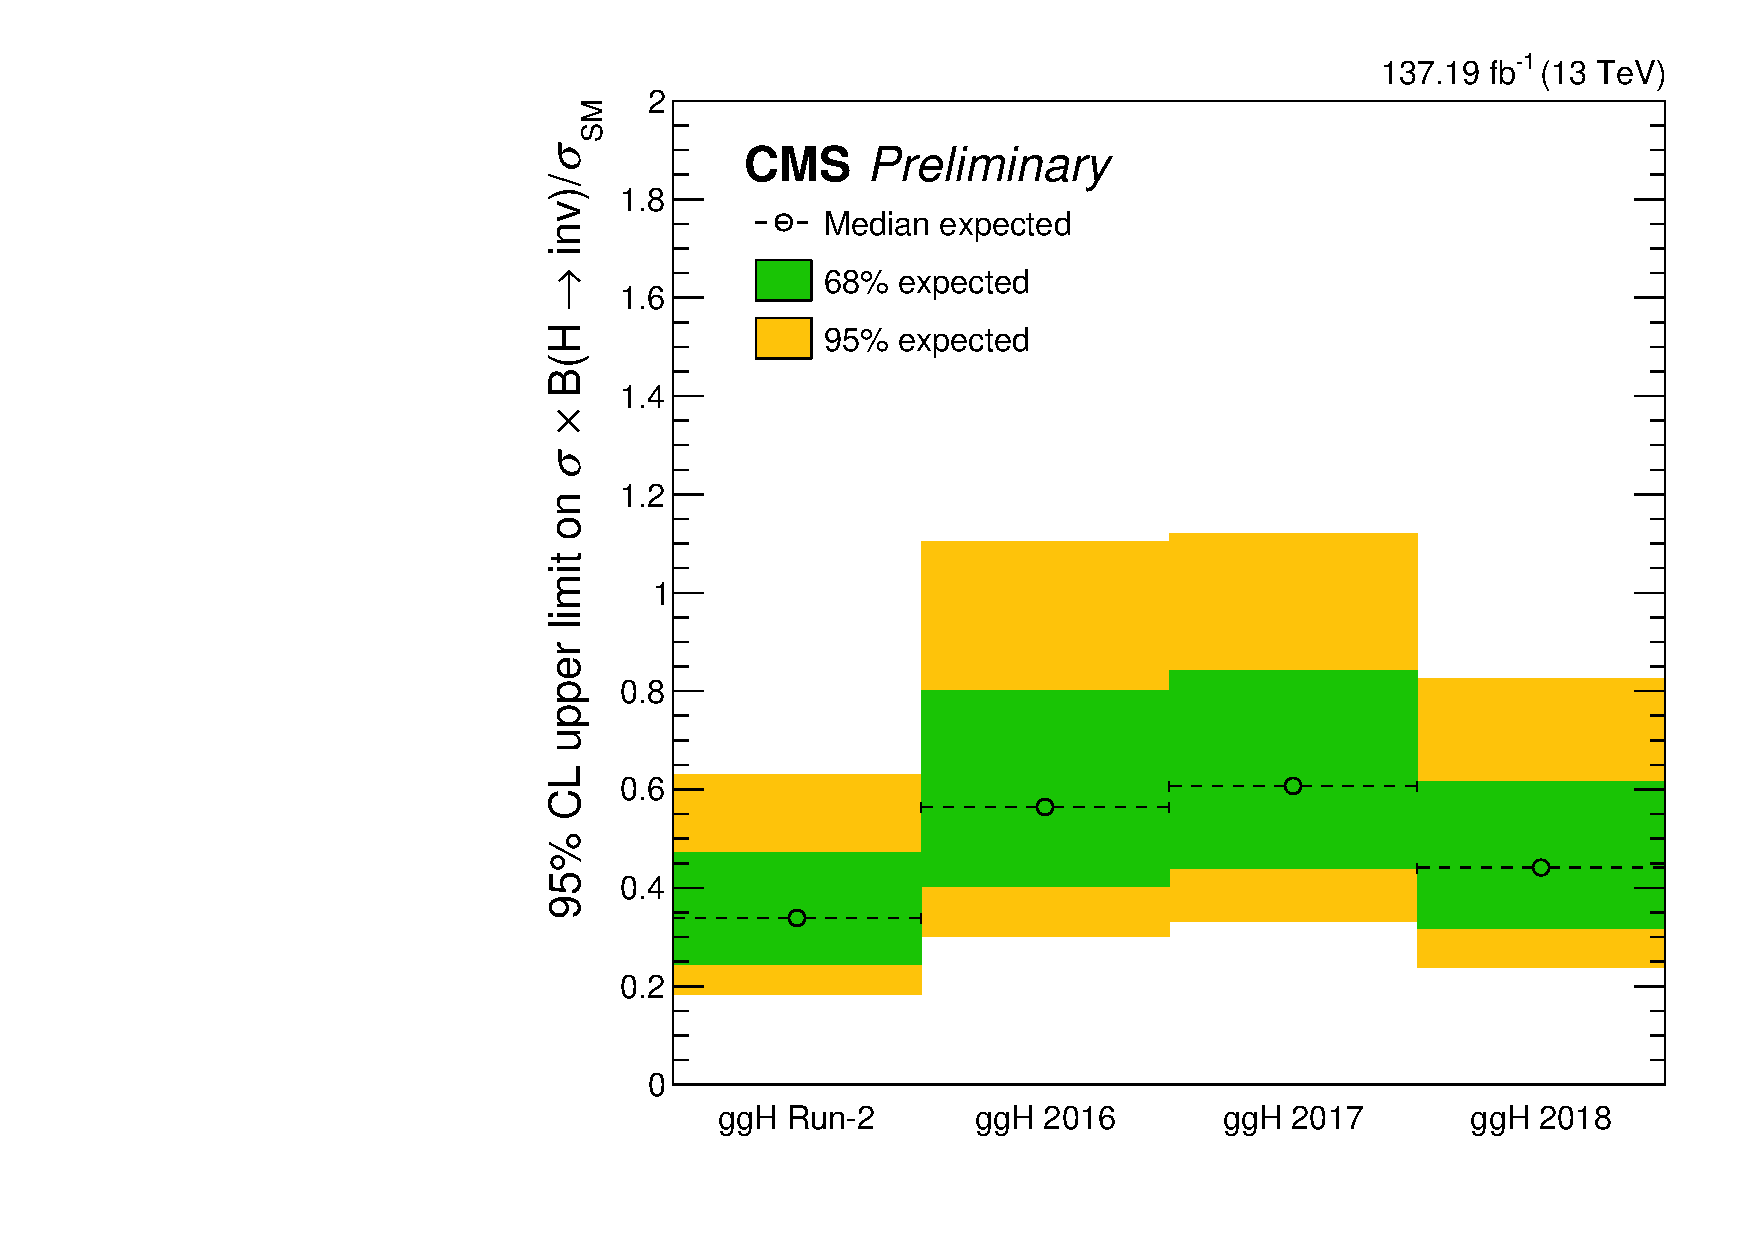
\includegraphics[width=\textwidth]{figures/limits/ggF/limit_Run2_ggF_Scenario5.pdf}
        \caption{\ggH --- Run-2}
    \end{subfigure}
    \caption[Expected 95\,\% CL upper limits on the Higgs boson to invisible state branching fraction in the \ggH category, for both the individual subcategories, and the combination of them, for each data-taking year in Run-2]{Expected 95\,\% CL upper limits on the Higgs boson to invisible state branching fraction in the \ggH category, for both the individual subcategories, and the combination of them, for each data-taking year in Run-2.}
    \label{fig:htoinv_limit_ggF}
\end{figure}


%=========================================================


\section{Combined results}
\label{sec:htoinv_combined_results}

% Show the results combined over all production modes (one plot for each year), then the full combination for Run-2, ideally with VBF results as well

Upper limits for $\BRof{\higgstoinv}$ by combining all categories for a given year are given for 2016, 2017, and 2018 in Figs.~\ref{fig:htoinv_limit_likelihood_2016}, \ref{fig:htoinv_limit_likelihood_2017}, \ref{fig:htoinv_limit_likelihood_2018}, respectively. For the full Run-2 dataset, they are broken down by data taking year in Fig.~\ref{fig:htoinv_limit_likelihood_Run2_per_year} and by category in Fig.~\ref{fig:htoinv_limit_likelihood_Run2_per_cat}.\footnote{Expected limits only, so far, and really only placeholders. The full Run-2 likelihood is not correct---fit fails to converge for most points.} Profile likelihood ratios as a function of $\BRof{\higgstoinv}$ are also presented opposite the limits.

\begin{figure}[htbp]
    \centering
    \begin{subfigure}[t]{0.45\textwidth}  % top align since figures are same dimensions, but x-axis labels are larger for likelihood
        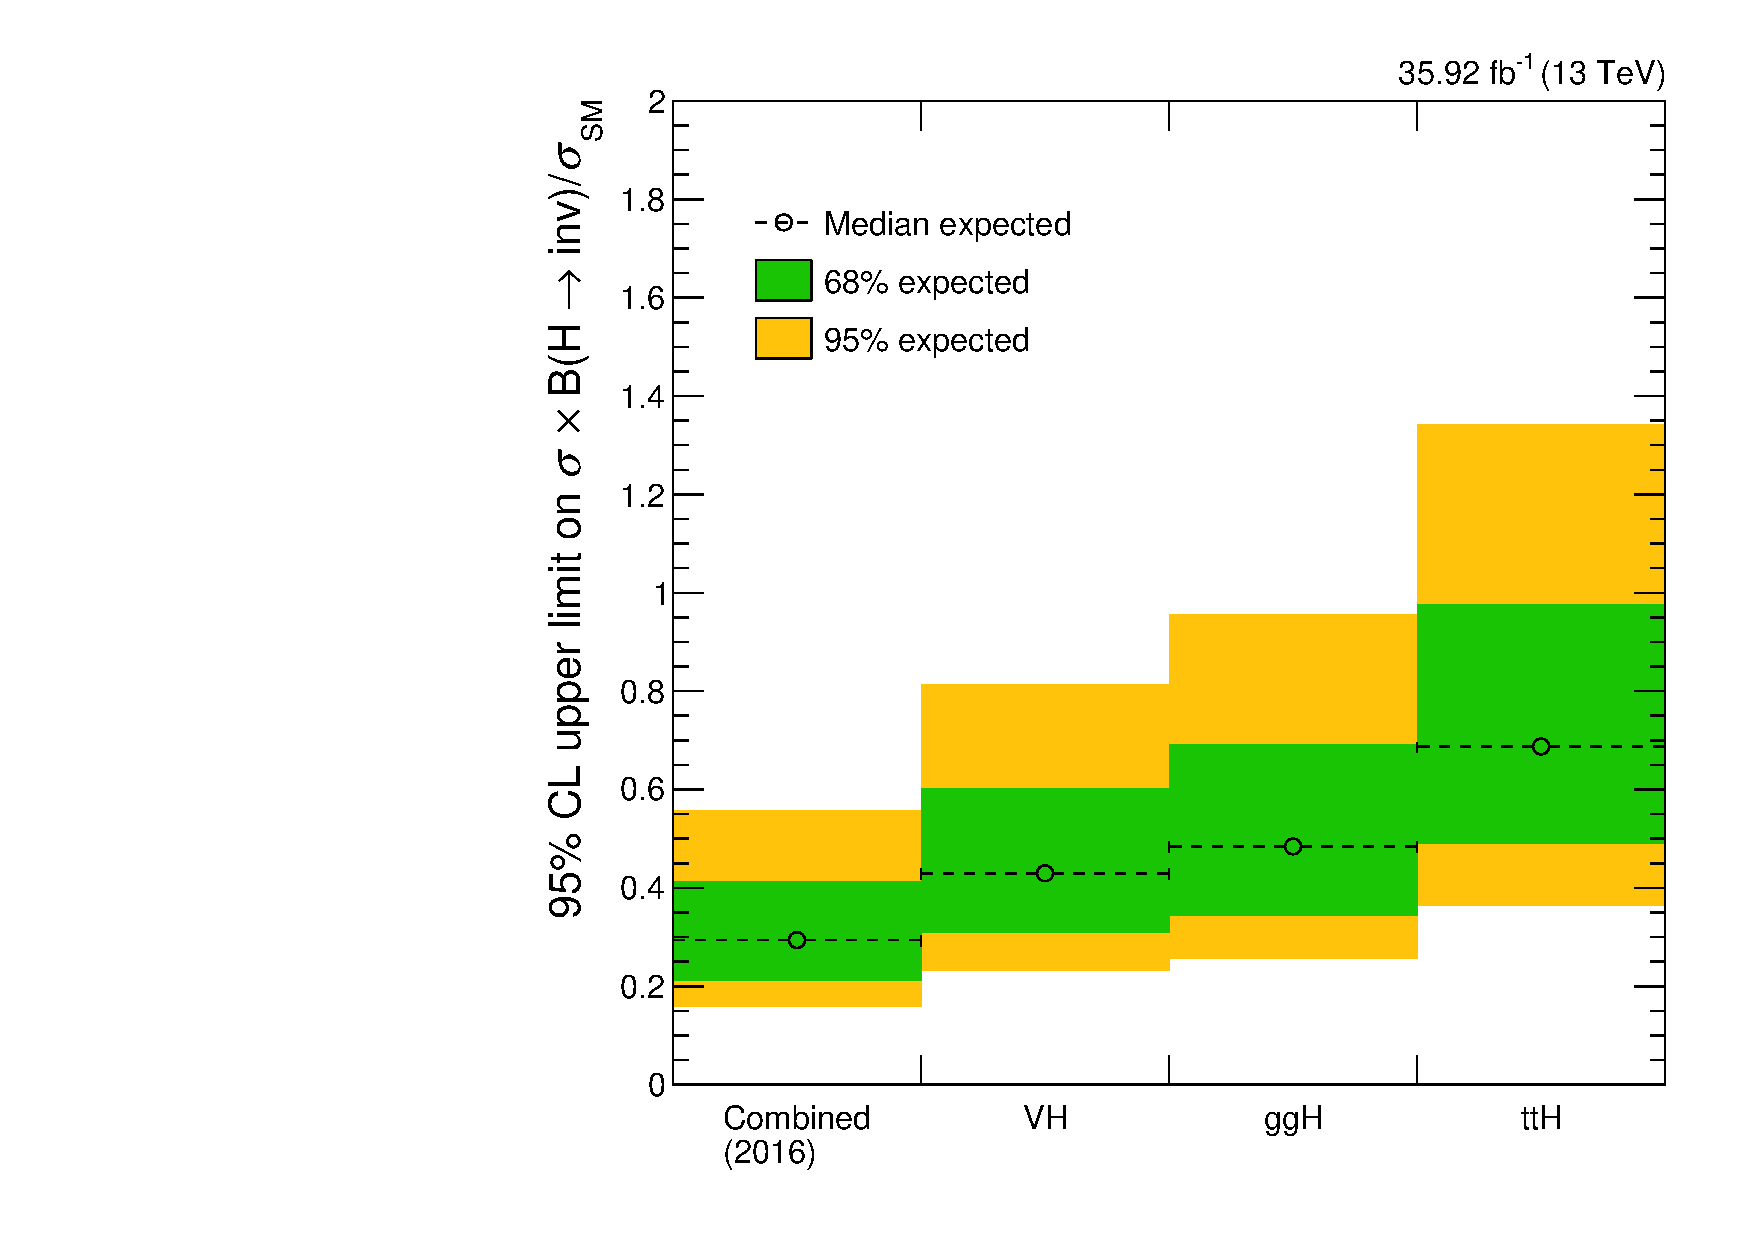
\includegraphics[width=\textwidth]{figures/limits/per_year/limit_2016_comb_Scenario5.pdf}
        \caption{Expected limit -- 2016}
    \end{subfigure}
    \hspace{0.05\textwidth}
    \begin{subfigure}[t]{0.45\textwidth}
        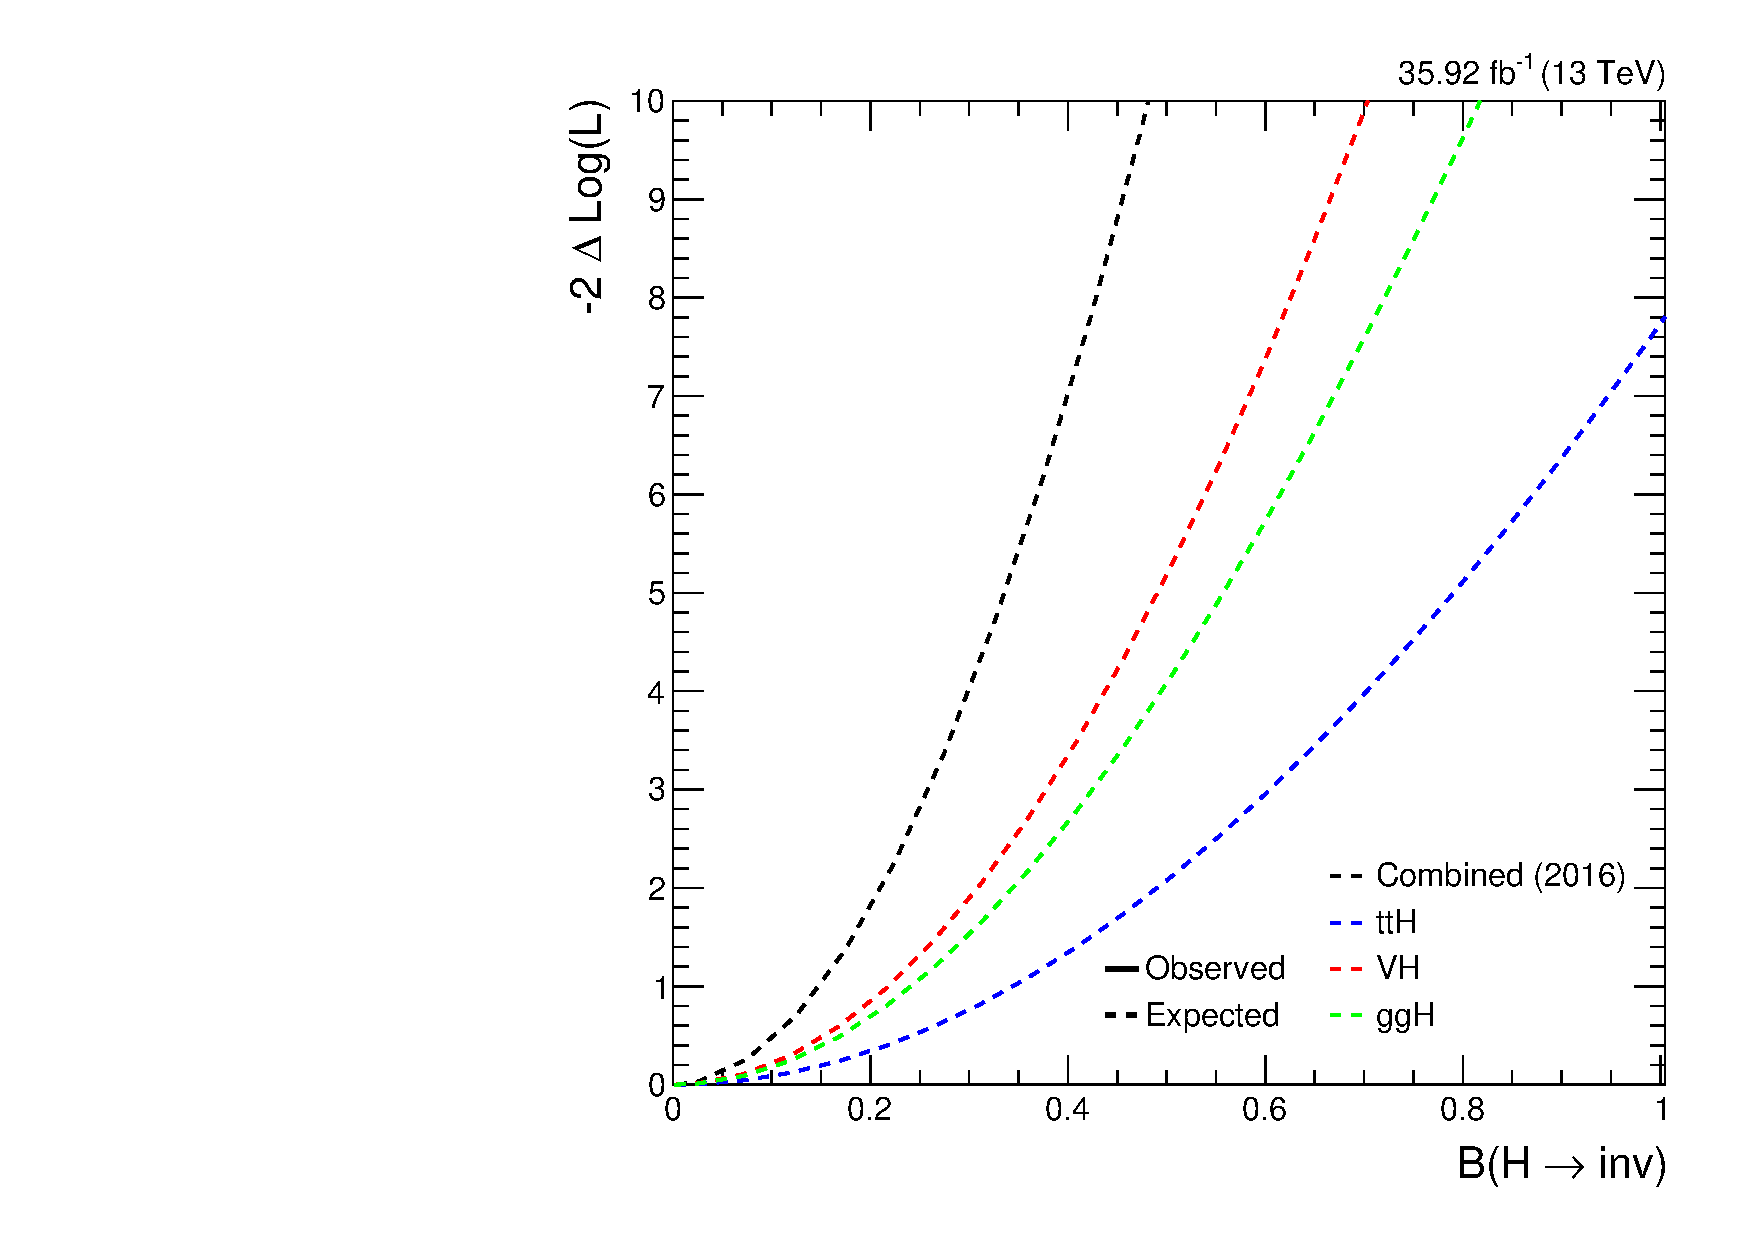
\includegraphics[width=\textwidth]{figures/likelihood_scan/profile_likelihood_scan_2016_Scenario5.pdf}
        \caption{Profile likelihood -- 2016}
    \end{subfigure}
    \caption[Expected 95\,\% CL upper limit on the Higgs boson to invisible state branching fraction $\BRof{\higgstoinv}$ and the corresponding profile likelihood ratio as a function of it, for both the individual categories that target a specific production mode, as well as the combination of them, for the 2016 dataset]{Expected 95\,\% CL upper limit on the Higgs boson to invisible state branching fraction $\BRof{\higgstoinv}$ (left) and the corresponding profile likelihood ratio as a function of it (right), for both the individual categories that target a specific production mode, as well as the combination of them, for the 2016 dataset. The \acrlong{sm} Higgs boson with its associated mass and production cross section are assumed.}
    \label{fig:htoinv_limit_likelihood_2016}
\end{figure}

\begin{figure}[htbp]
    \centering
    \begin{subfigure}[t]{0.45\textwidth}
        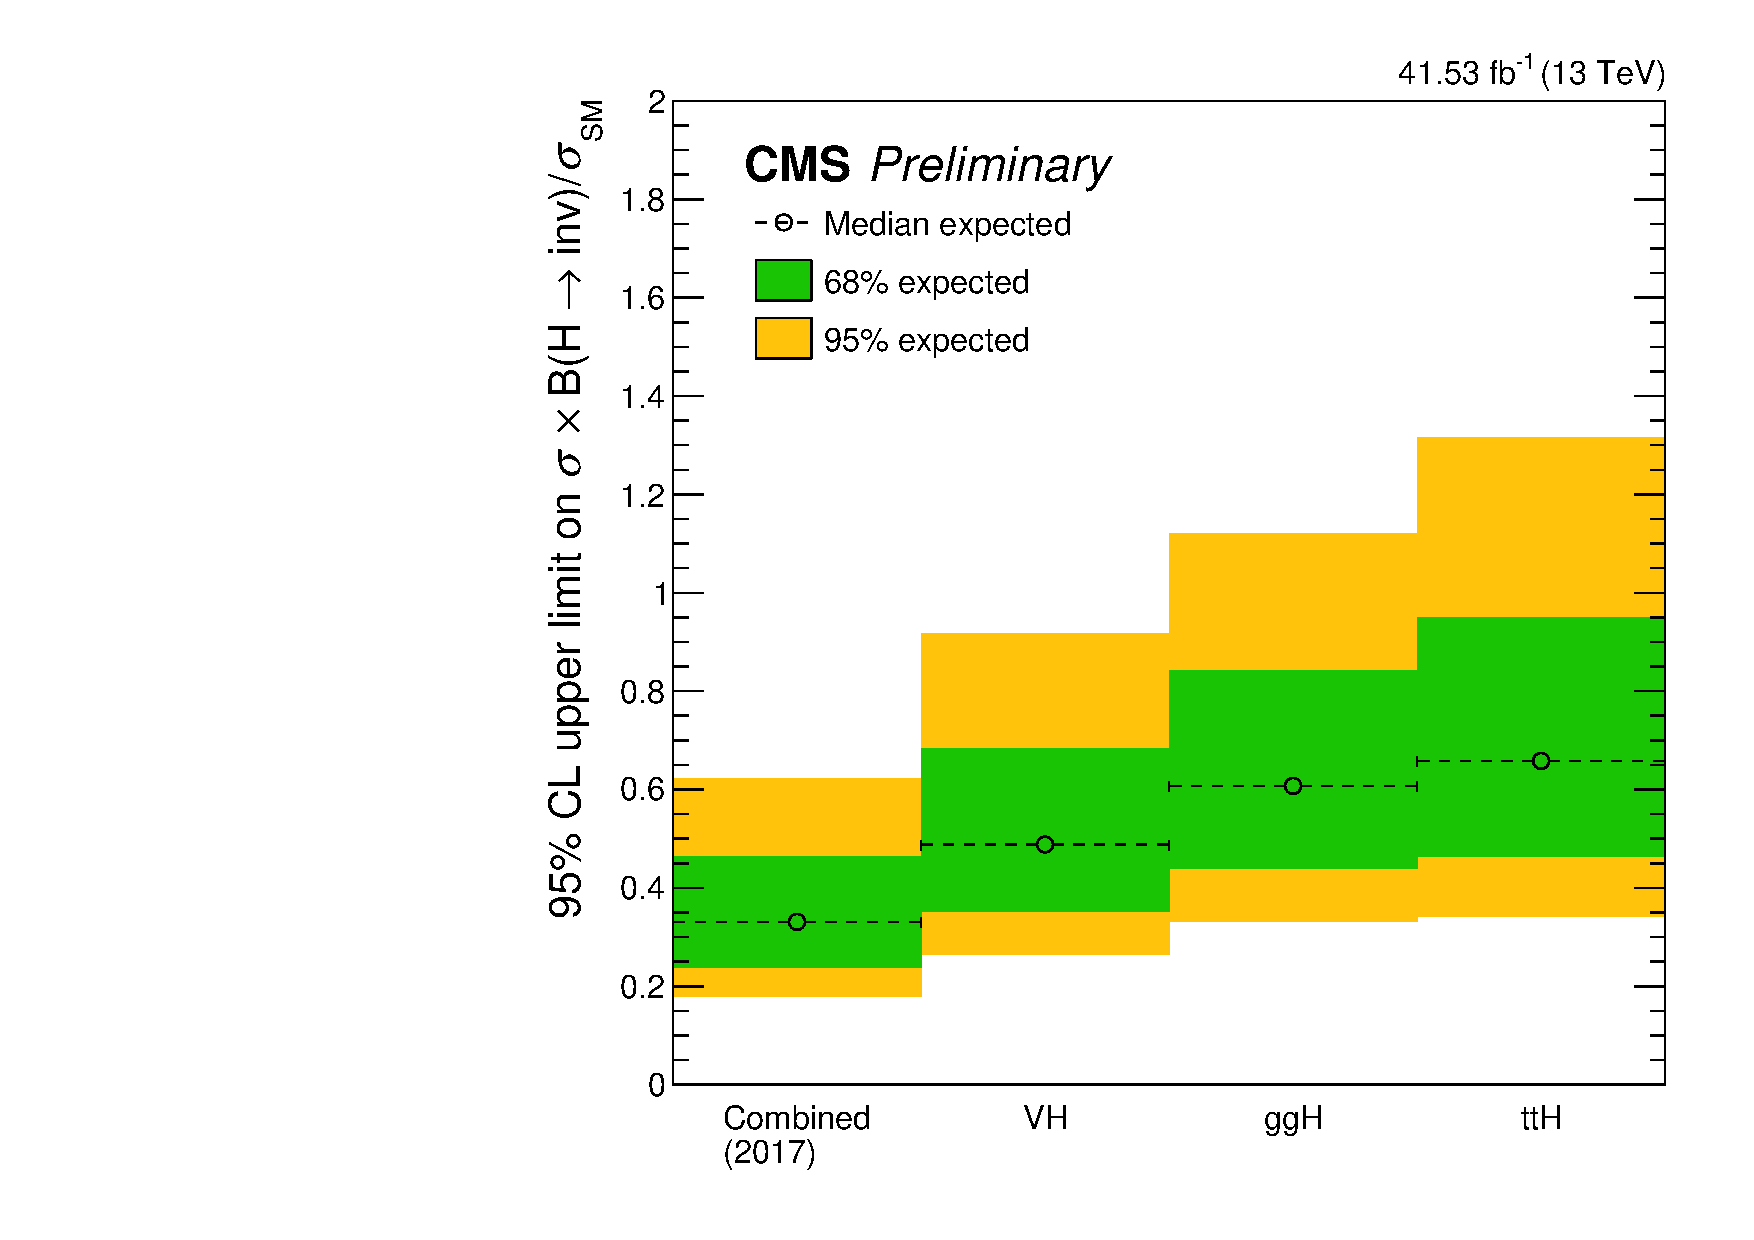
\includegraphics[width=\textwidth]{figures/limits/per_year/limit_2017_comb_Scenario5.pdf}
        \caption{Expected limit -- 2017}
    \end{subfigure}
    \hspace{0.05\textwidth}
    \begin{subfigure}[t]{0.45\textwidth}
        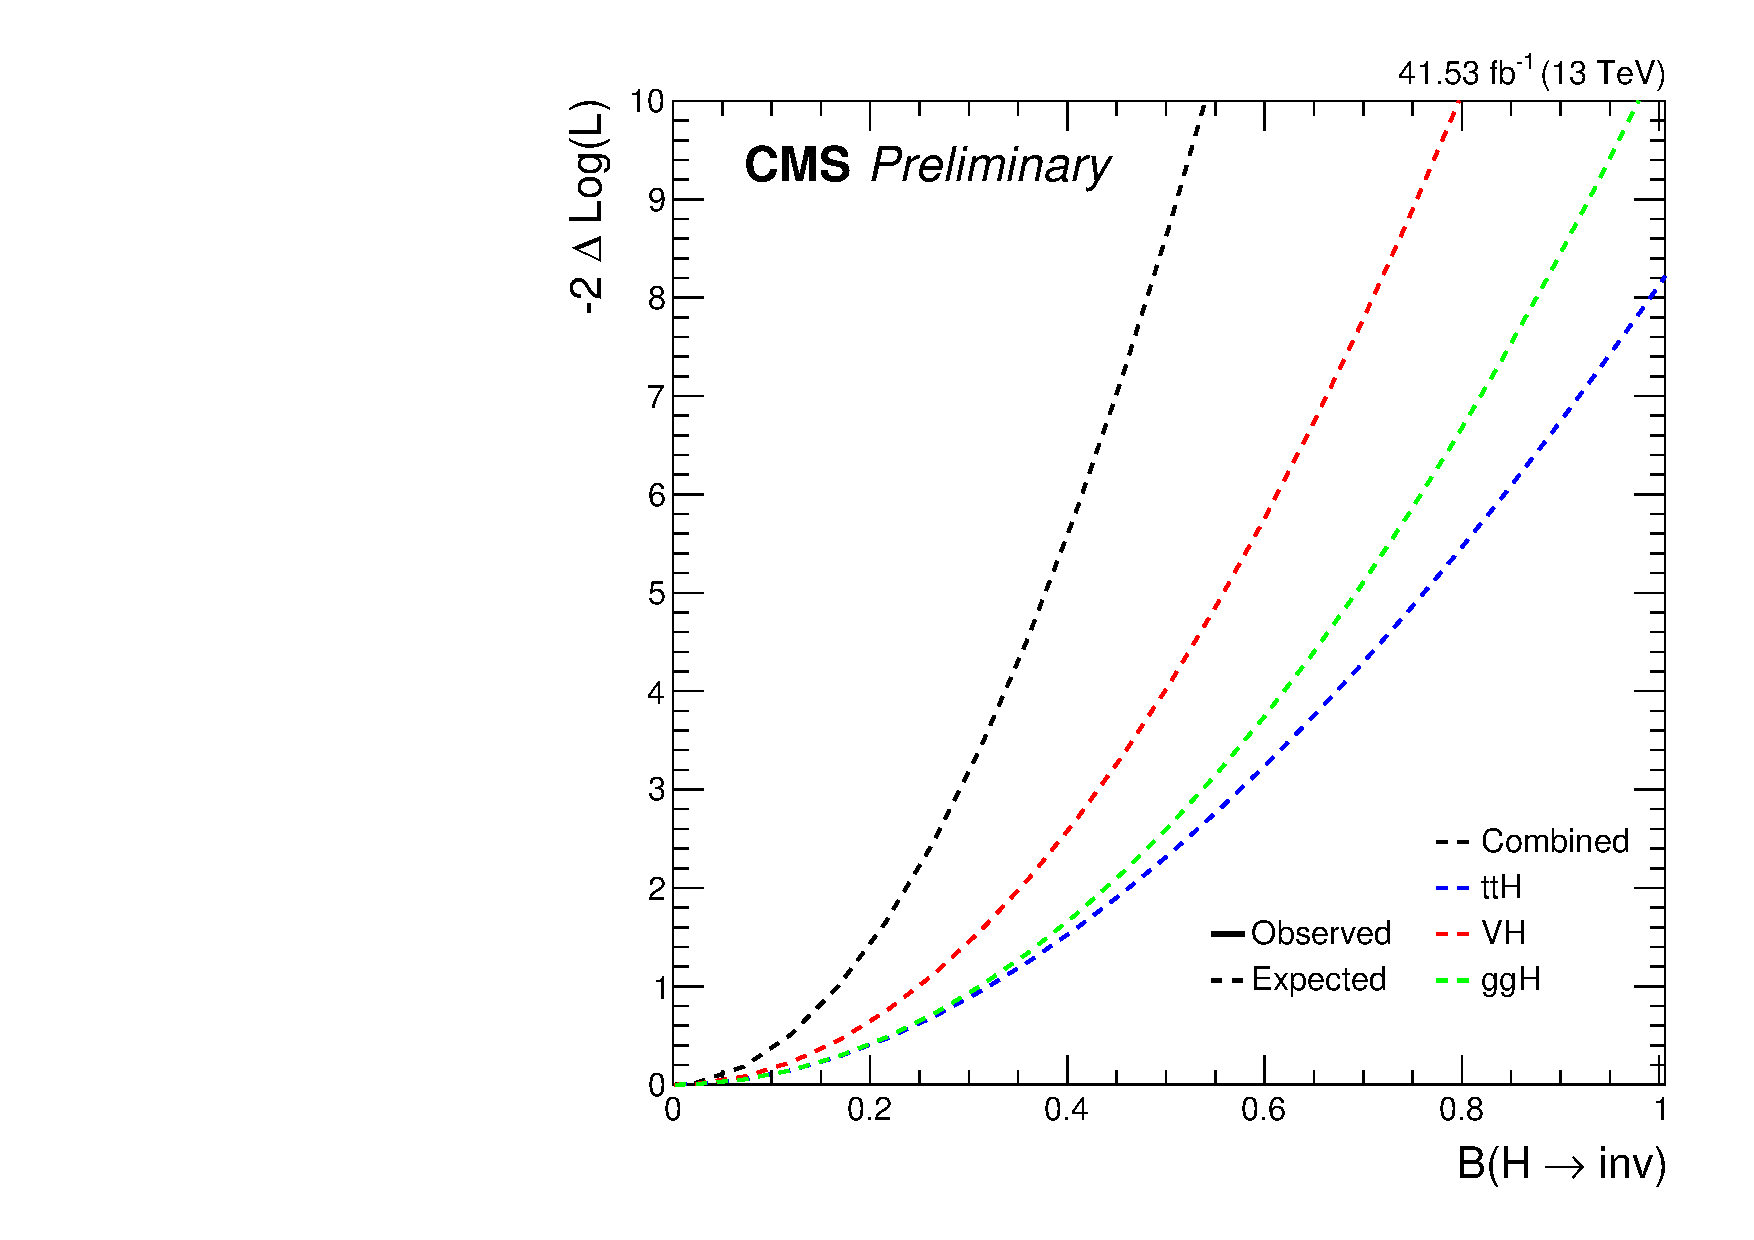
\includegraphics[width=\textwidth]{figures/likelihood_scan/profile_likelihood_scan_2017_Scenario5.pdf}
        \caption{Profile likelihood -- 2017}
    \end{subfigure}
    \caption[Expected 95\,\% CL upper limit on the Higgs boson to invisible state branching fraction $\BRof{\higgstoinv}$ and the corresponding profile likelihood ratio as a function of it, for both the individual categories that target a specific production mode, as well as the combination of them, for the 2017 dataset]{Expected 95\,\% CL upper limit on the Higgs boson to invisible state branching fraction $\BRof{\higgstoinv}$ (left) and the corresponding profile likelihood ratio as a function of it (right), for both the individual categories that target a specific production mode, as well as the combination of them, for the 2017 dataset. The \acrlong{sm} Higgs boson with its associated mass and production cross section are assumed.}
    \label{fig:htoinv_limit_likelihood_2017}
\end{figure}

\begin{figure}[htbp]
    \centering
    \begin{subfigure}[t]{0.45\textwidth}
        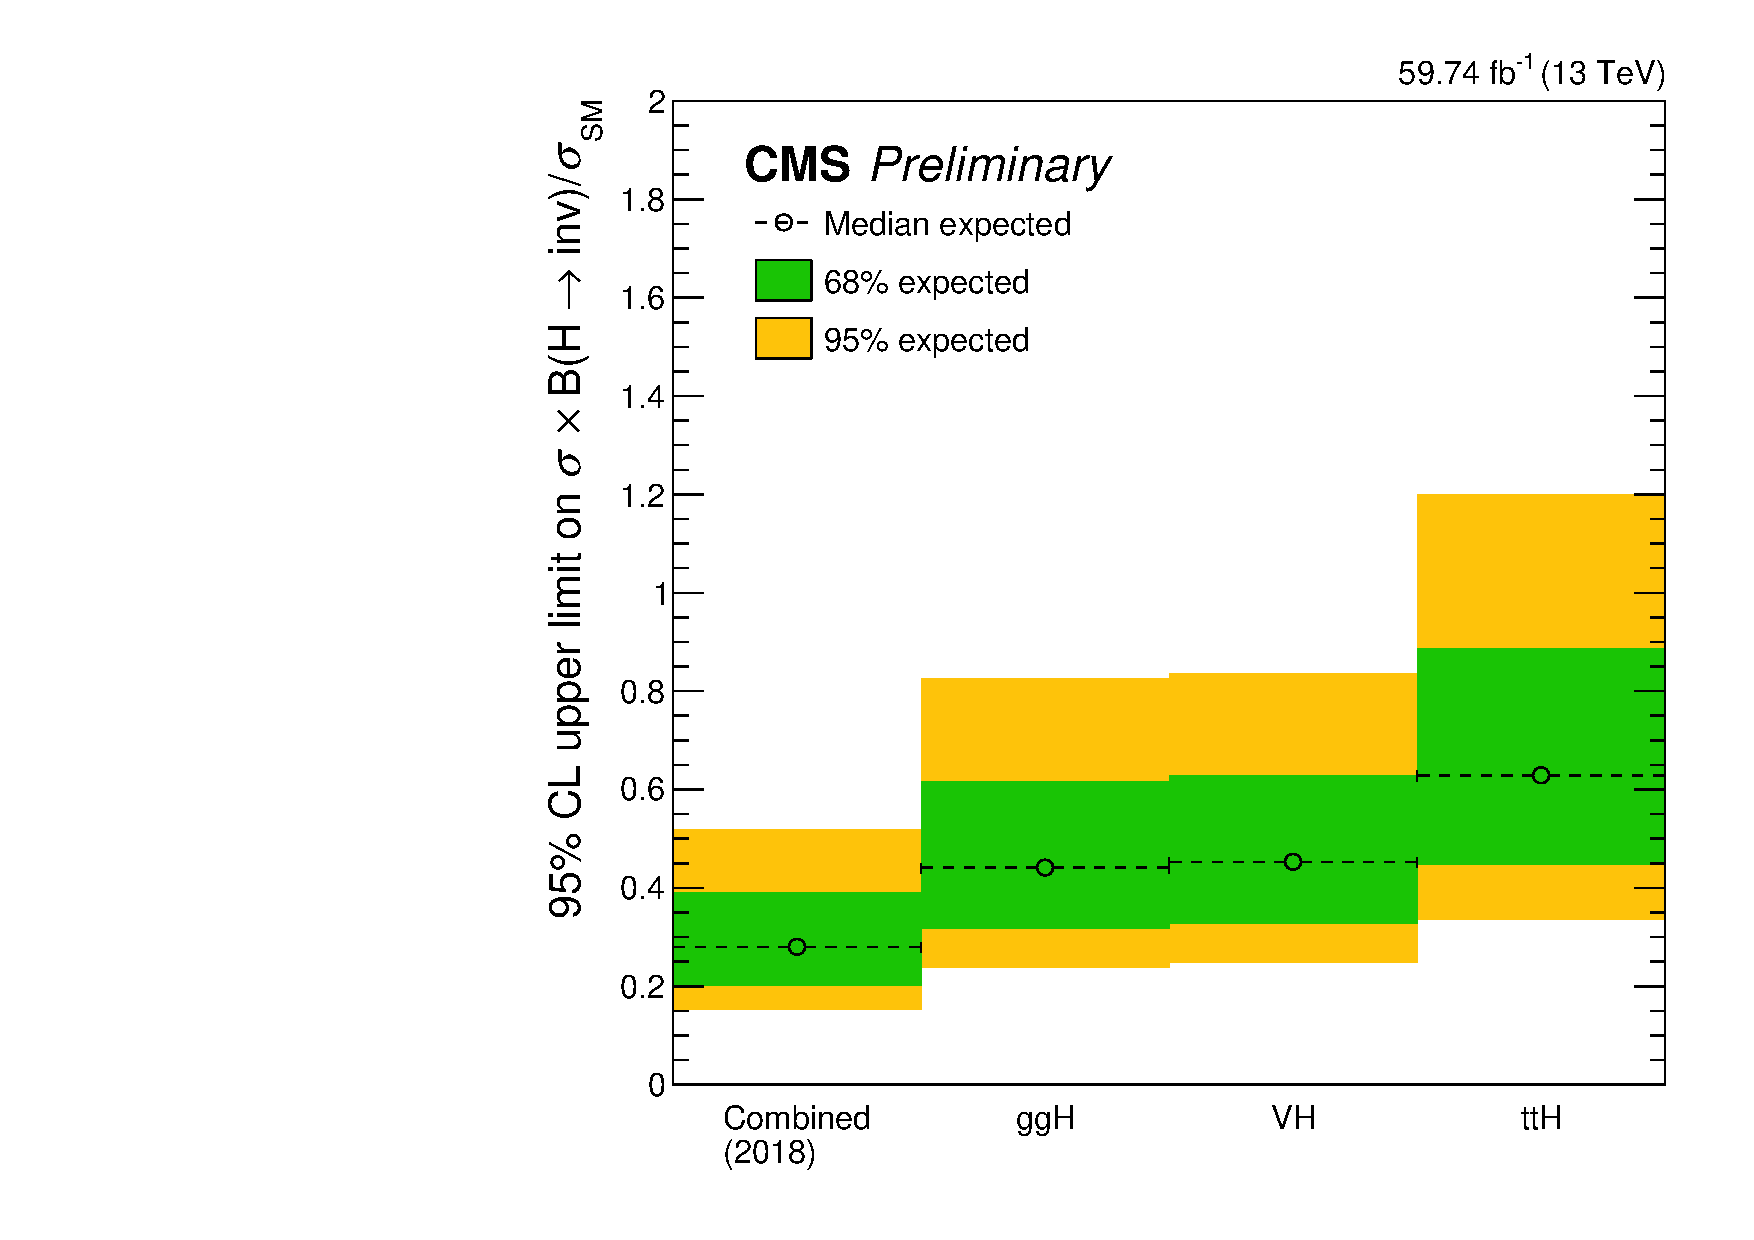
\includegraphics[width=\textwidth]{figures/limits/per_year/limit_2018_comb_Scenario5.pdf}
        \caption{Expected limit -- 2018}
    \end{subfigure}
    \hspace{0.05\textwidth}
    \begin{subfigure}[t]{0.45\textwidth}
        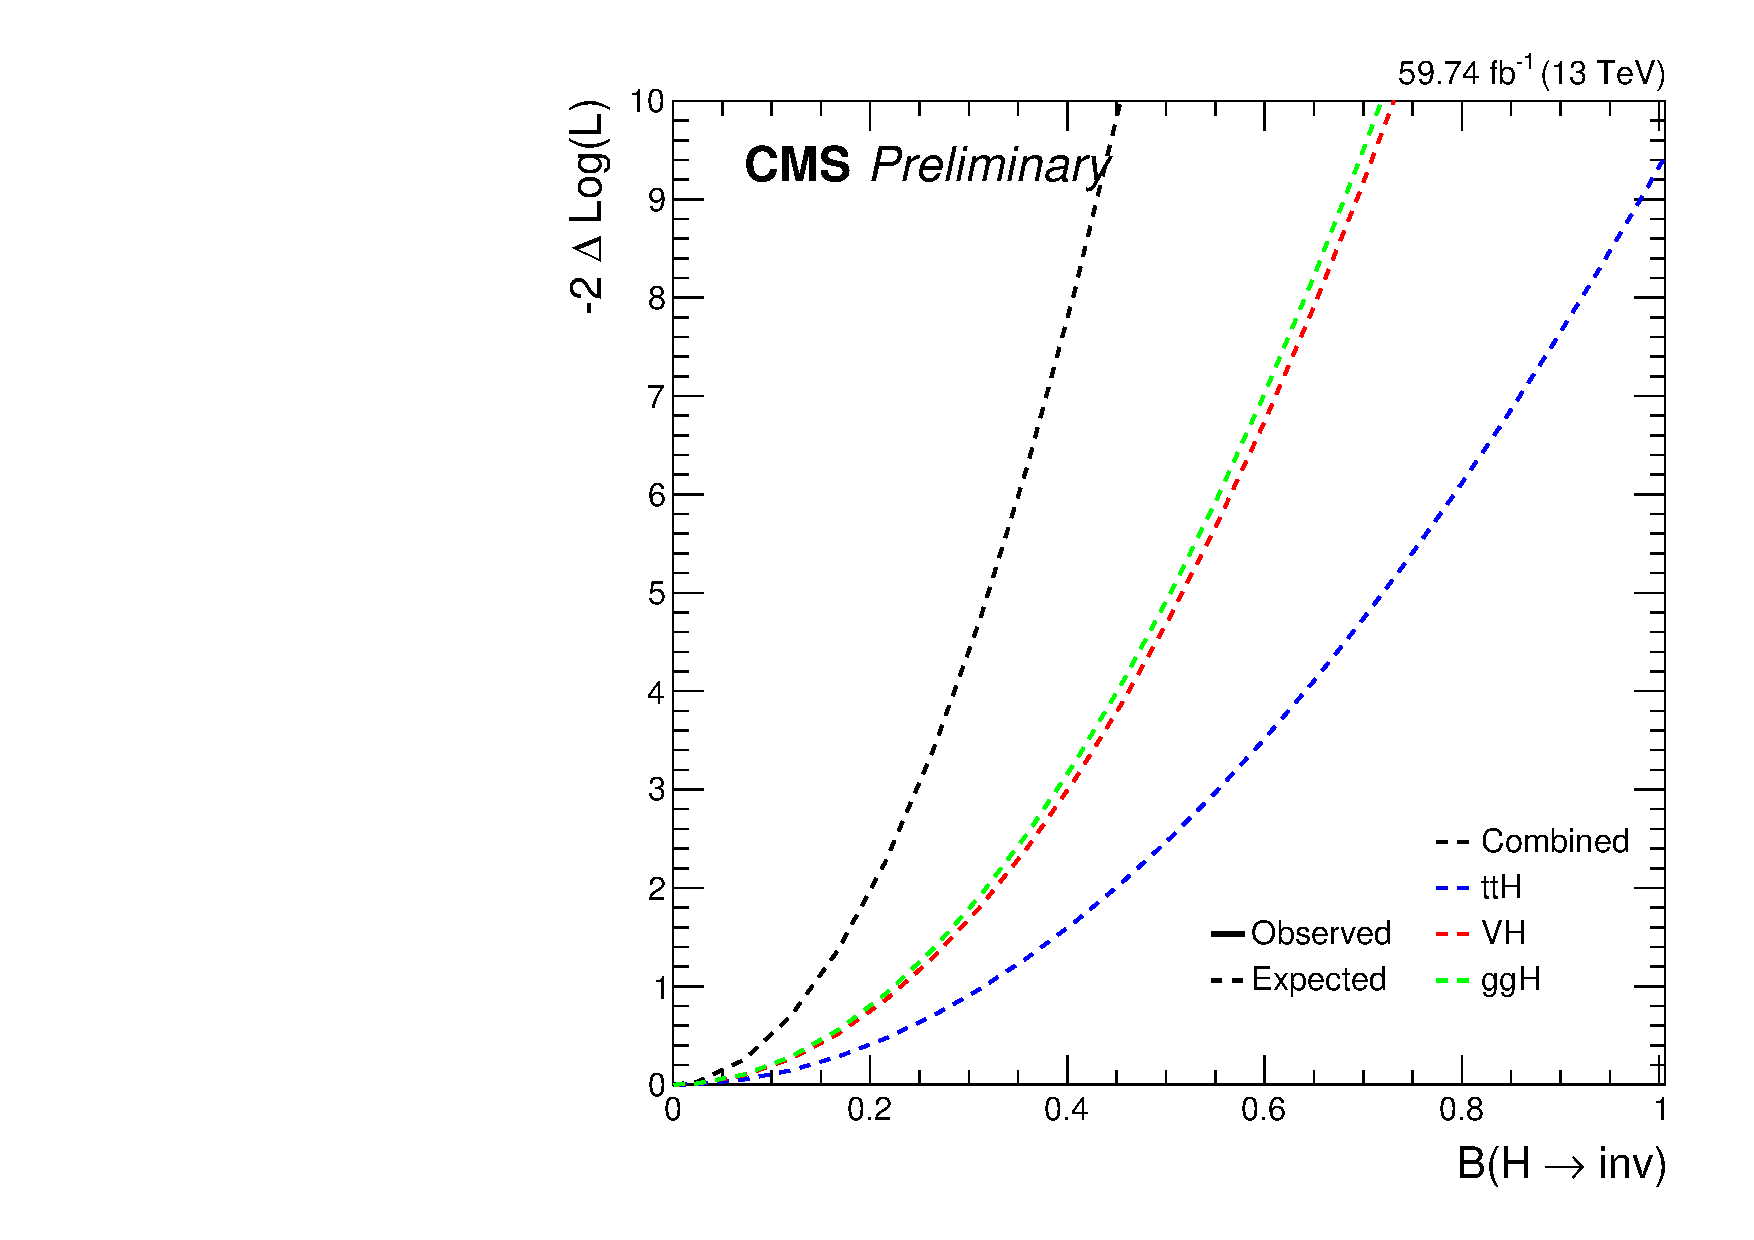
\includegraphics[width=\textwidth]{figures/likelihood_scan/profile_likelihood_scan_2018_Scenario5.pdf}
        \caption{Profile likelihood -- 2018}
    \end{subfigure}
    \caption[Expected 95\,\% CL upper limit on the Higgs boson to invisible state branching fraction $\BRof{\higgstoinv}$ and the corresponding profile likelihood ratio as a function of it, for both the individual categories that target a specific production mode, as well as the combination of them, for the 2018 dataset]{Expected 95\,\% CL upper limit on the Higgs boson to invisible state branching fraction $\BRof{\higgstoinv}$ (left) and the corresponding profile likelihood ratio as a function of it (right), for both the individual categories that target a specific production mode, as well as the combination of them, for the 2018 dataset. The \acrlong{sm} Higgs boson with its associated mass and production cross section are assumed.}
    \label{fig:htoinv_limit_likelihood_2018}
\end{figure}

\begin{figure}[htbp]
    \centering
    \begin{subfigure}[t]{0.45\textwidth}
        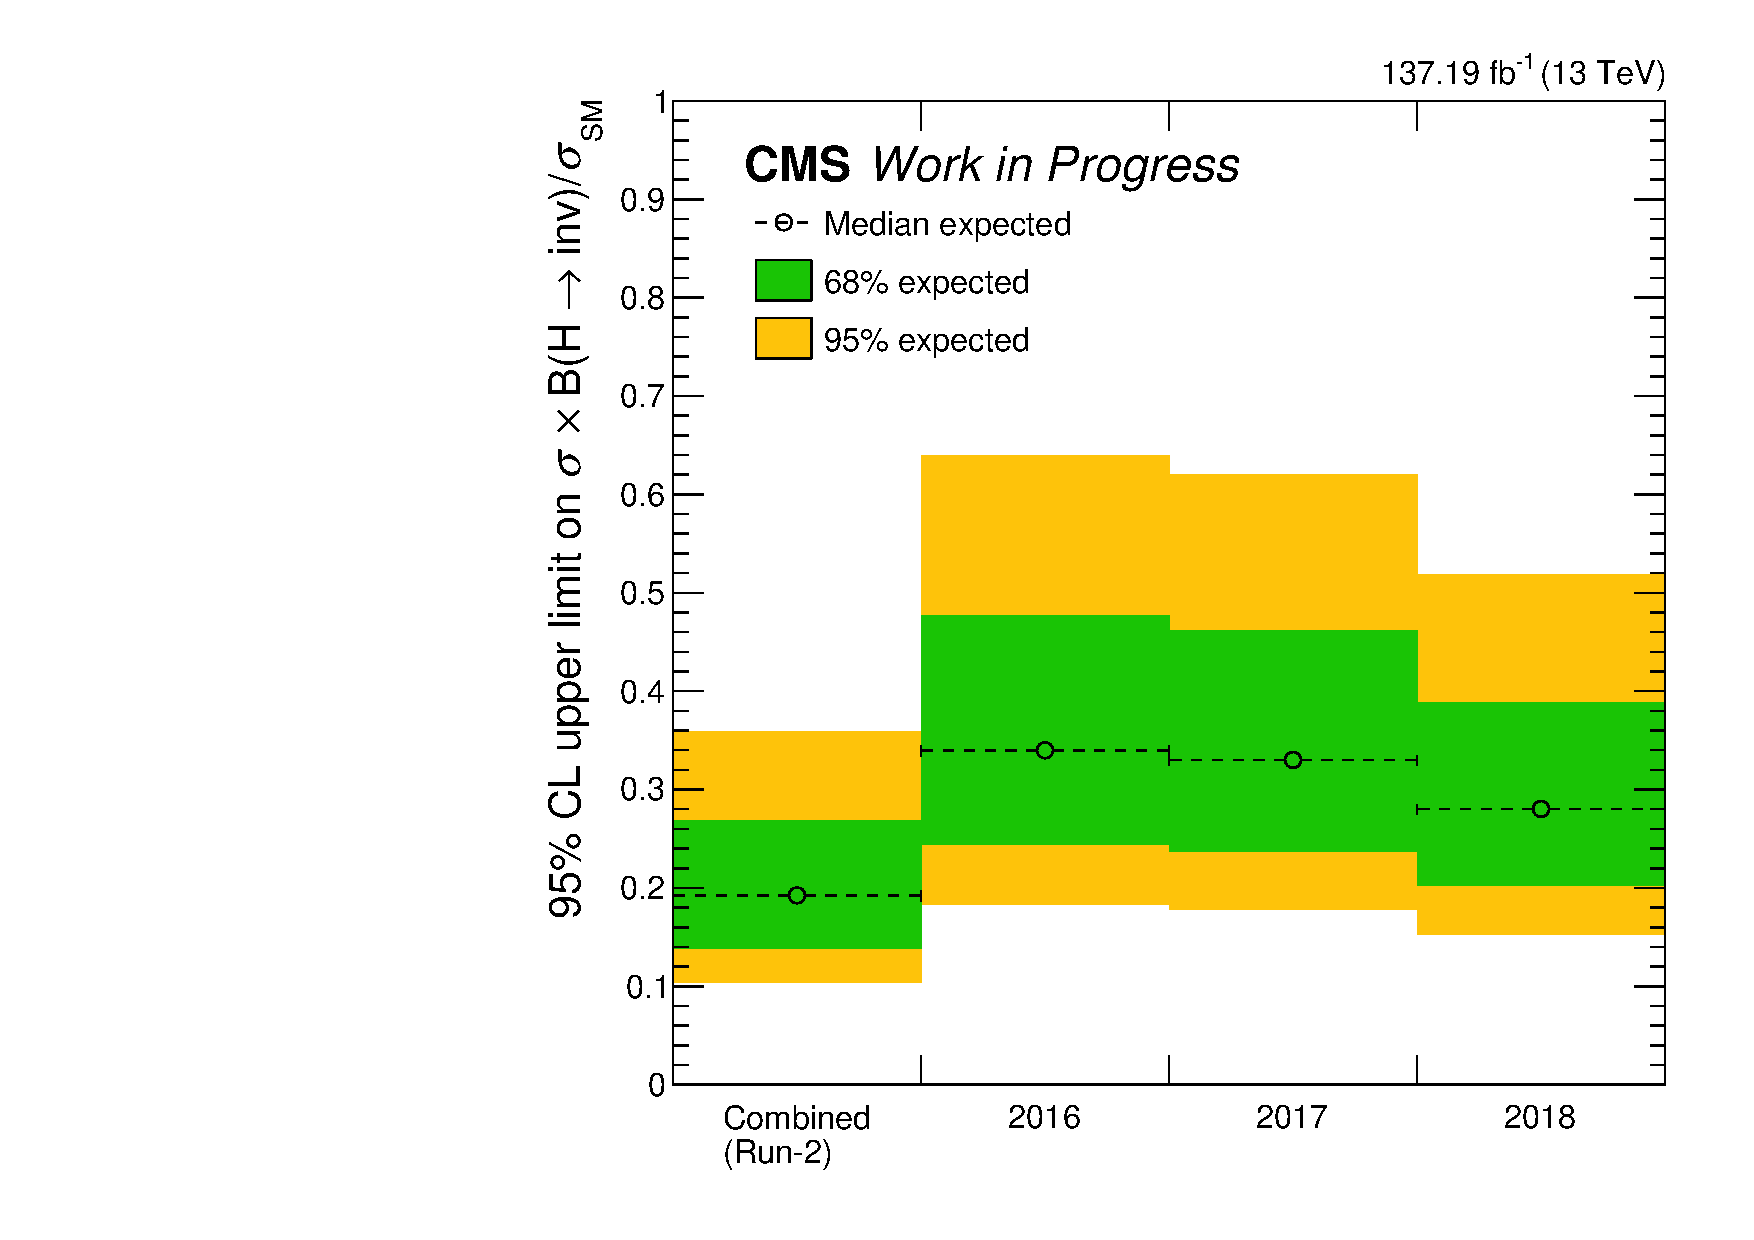
\includegraphics[width=\textwidth]{figures/limits/full_Run2/limit_Run2_comb_per_year_Scenario5.pdf}
        \caption{Expected limit -- Run-2}
    \end{subfigure}
    \hspace{0.05\textwidth}
    \begin{subfigure}[t]{0.45\textwidth}
        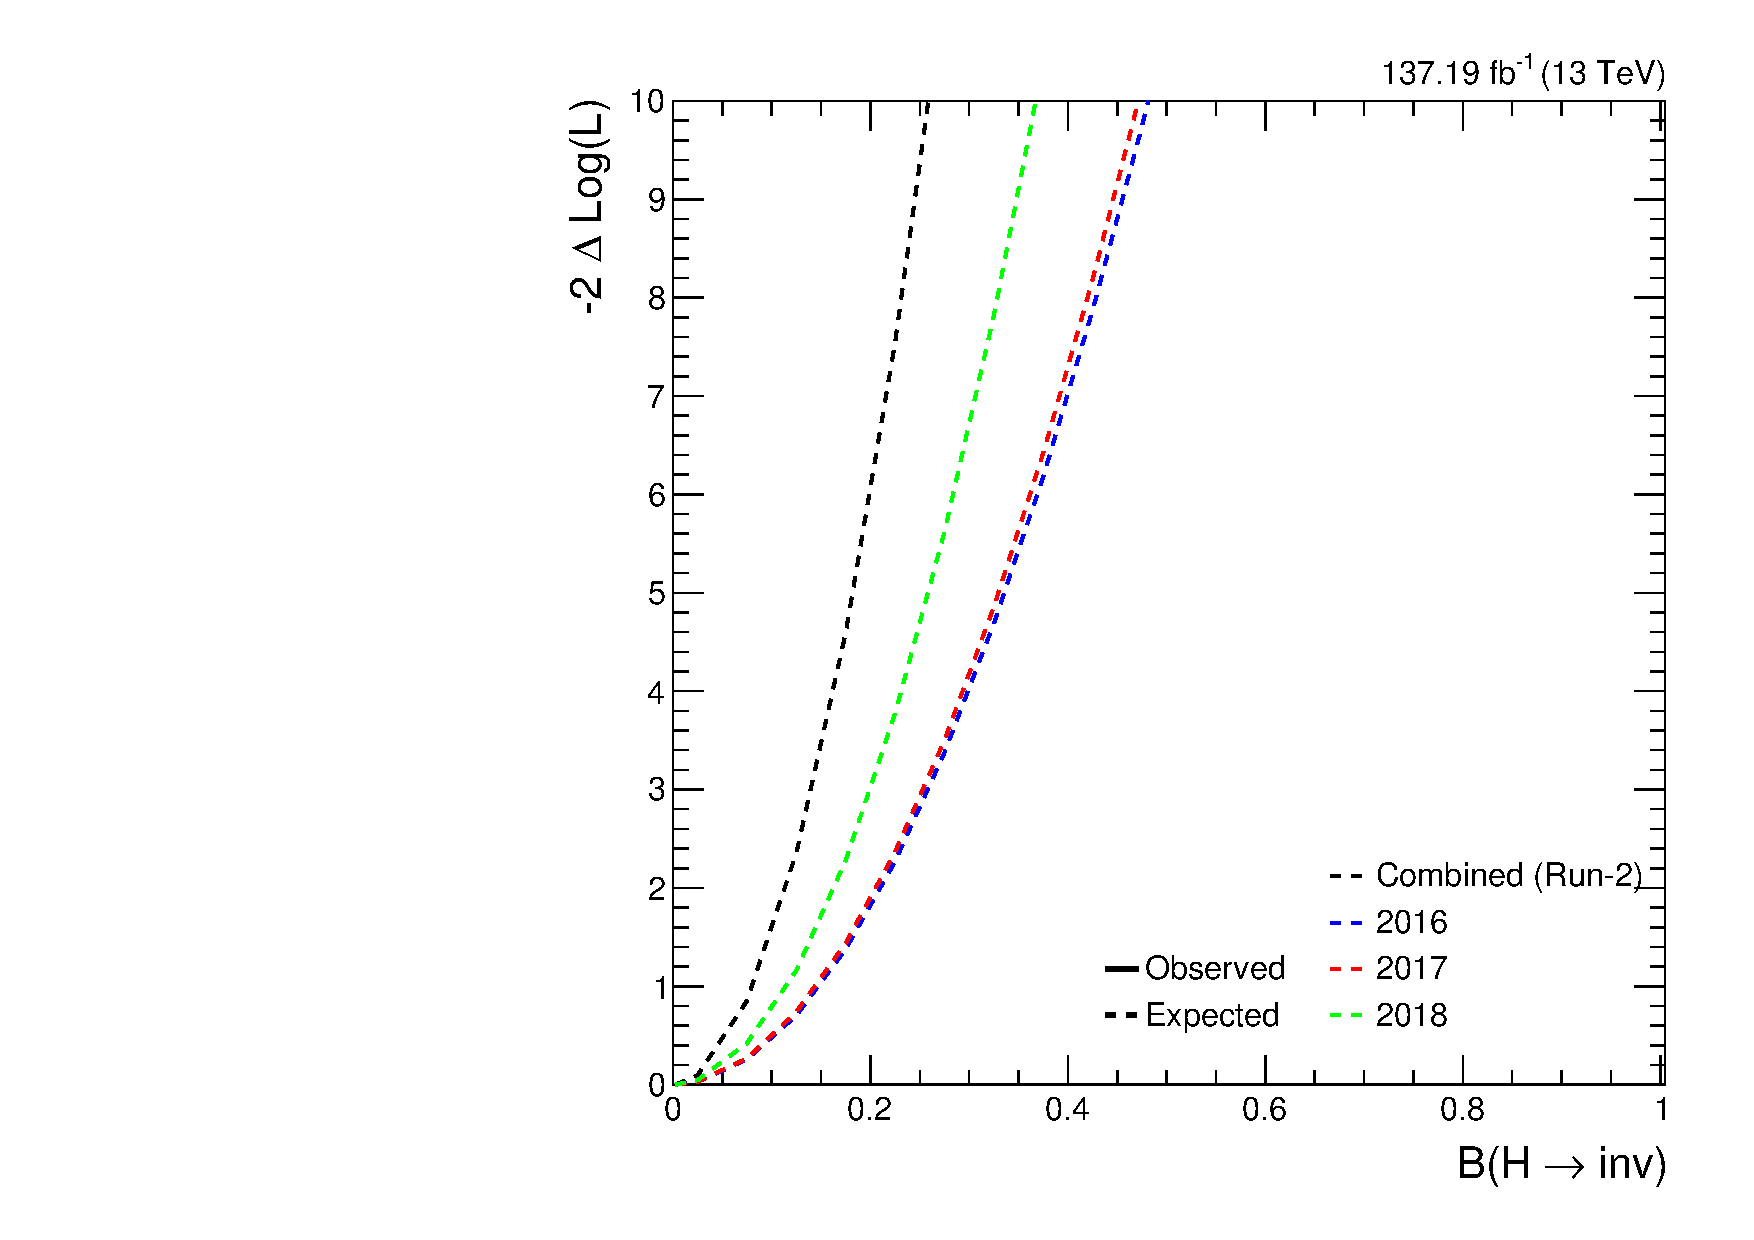
\includegraphics[width=\textwidth]{figures/likelihood_scan/profile_likelihood_scan_Run2_per_year_Scenario5.pdf}
        \caption{Profile likelihood -- Run-2}
    \end{subfigure}
    \caption[Expected 95\,\% CL upper limit on the Higgs boson to invisible state branching fraction $\BRof{\higgstoinv}$ and the corresponding profile likelihood ratio as a function of it, for both the individual data taking years, as well as the combination of them, for the full Run-2 dataset]{Expected 95\,\% CL upper limit on the Higgs boson to invisible state branching fraction $\BRof{\higgstoinv}$ (left) and the corresponding profile likelihood ratio as a function of it (right), for both the individual data taking years, as well as the combination of them, for the full Run-2 dataset. The \acrlong{sm} Higgs boson with its associated mass and production cross section are assumed.}
    \label{fig:htoinv_limit_likelihood_Run2_per_year}
\end{figure}

\begin{figure}[htbp]
    \centering
    \begin{subfigure}[b]{0.45\textwidth}  % top align since axis labels are larger for likelihood
        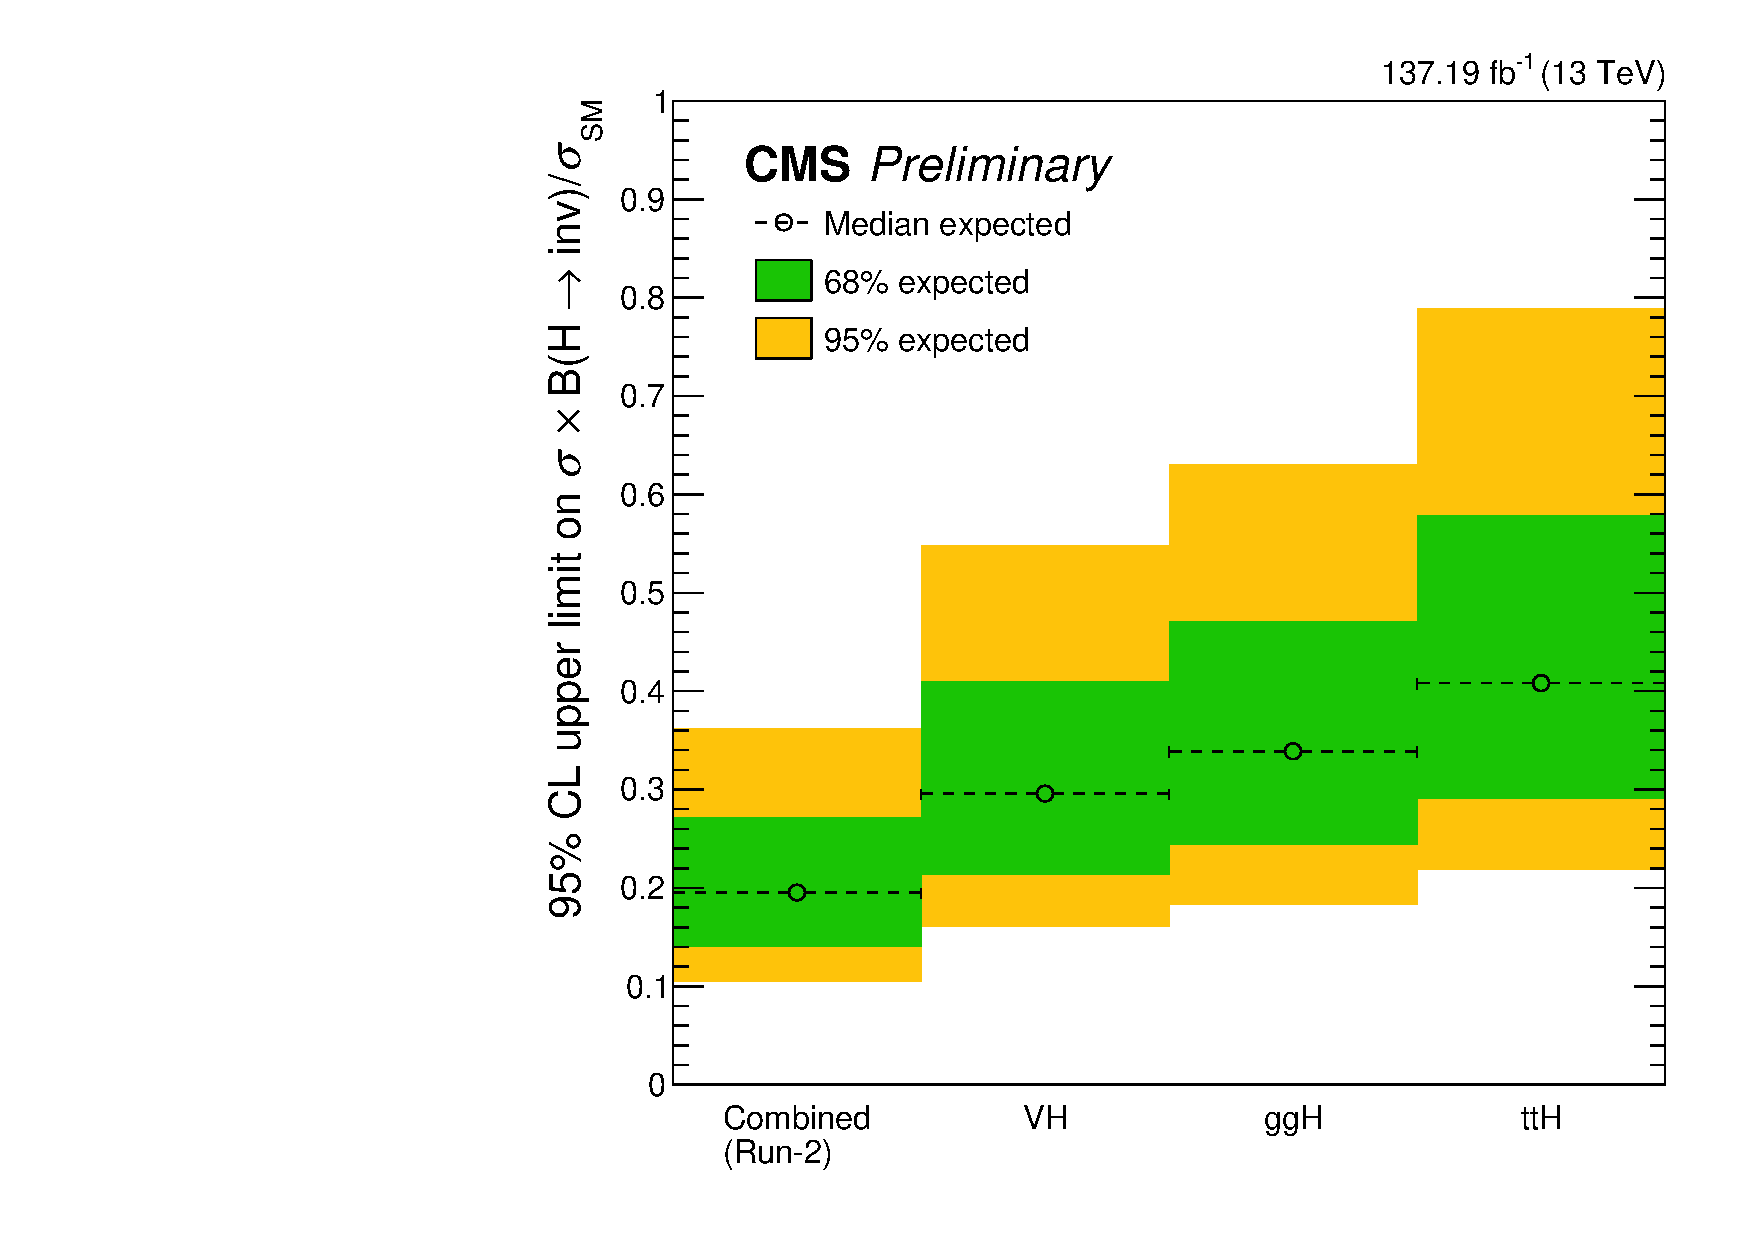
\includegraphics[width=\textwidth]{figures/limits/full_Run2/limit_Run2_comb_per_cat_Scenario5.pdf}
        \caption{Expected limit -- Run-2}
    \end{subfigure}
    \hspace{0.05\textwidth}
    \begin{subfigure}[b]{0.45\textwidth}
        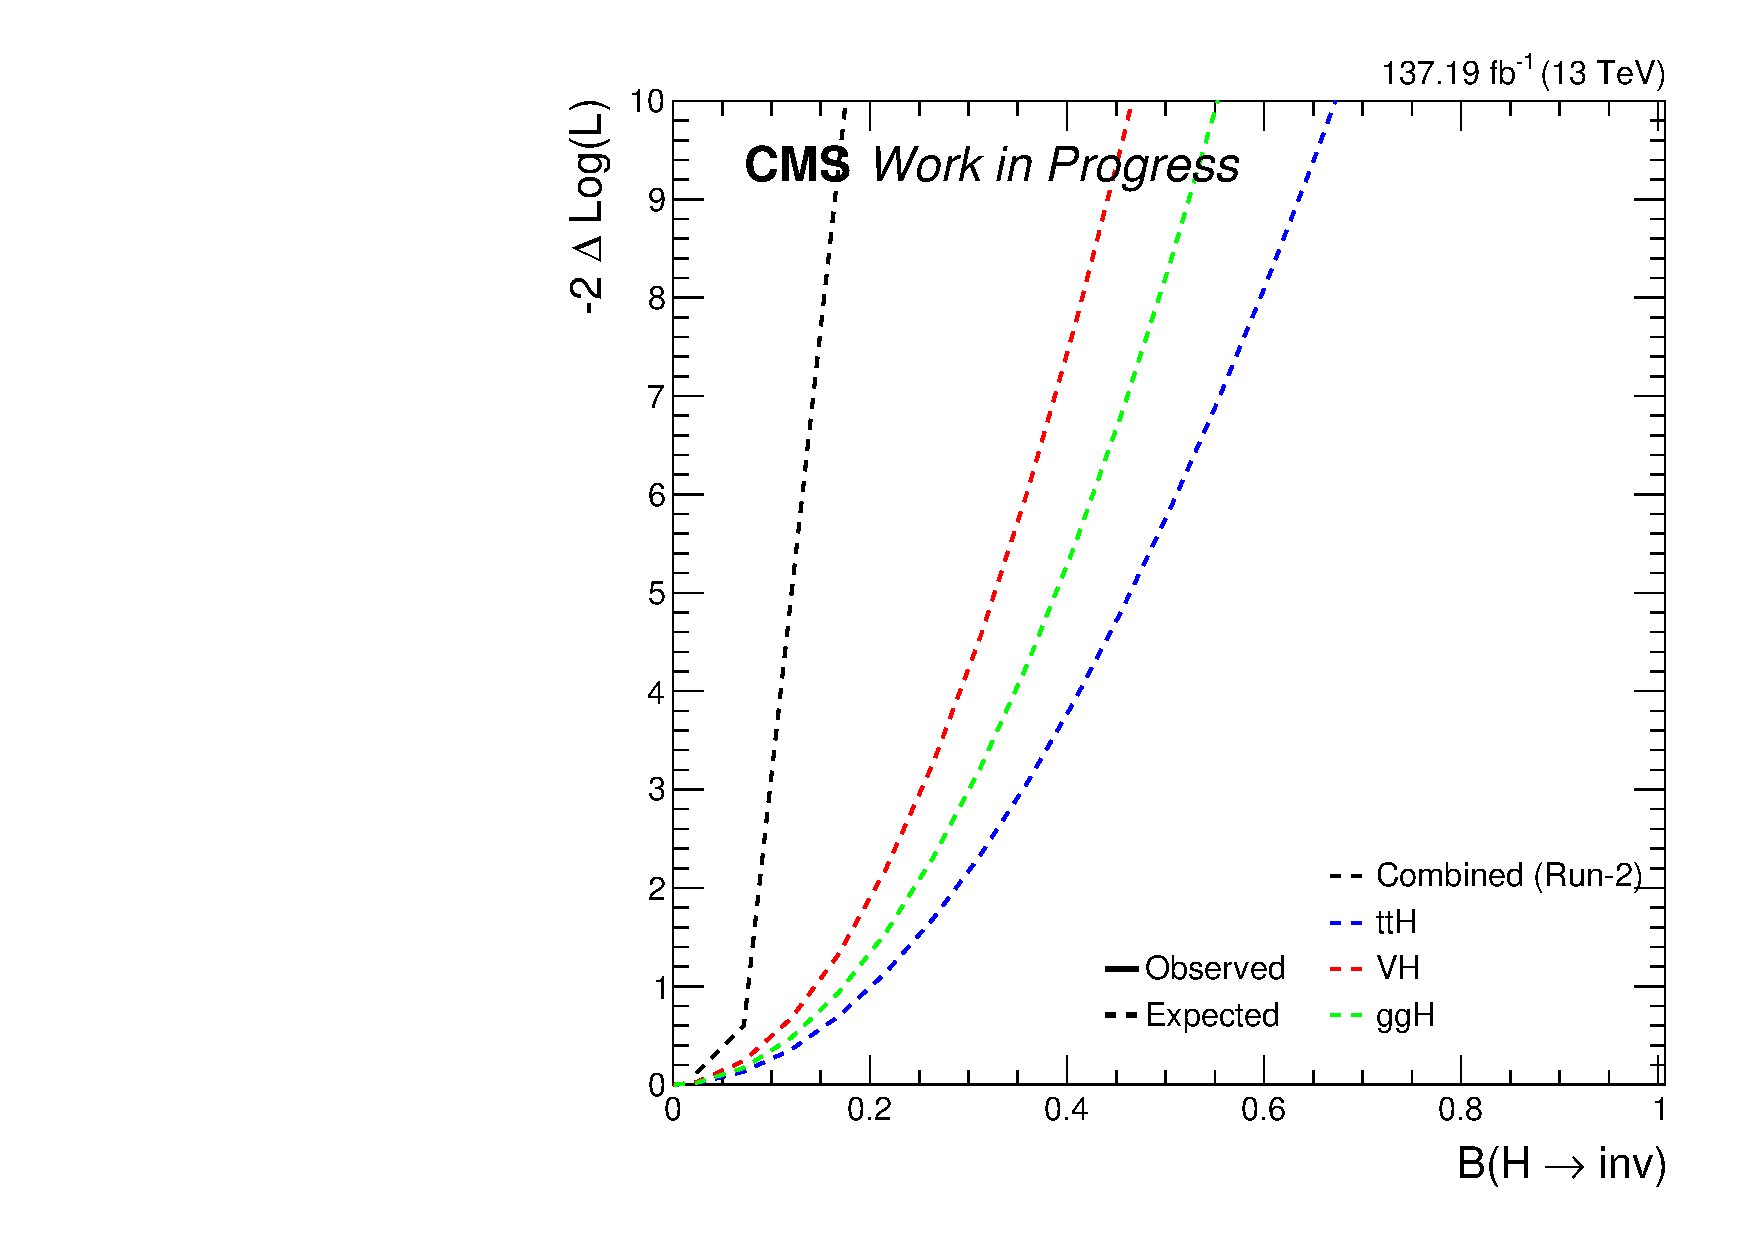
\includegraphics[width=\textwidth]{figures/likelihood_scan/profile_likelihood_scan_Run2_per_cat_Scenario5.pdf}
        \caption{Profile likelihood -- Run-2}
    \end{subfigure}
    \caption[Expected 95\,\% CL upper limit on the Higgs boson to invisible state branching fraction $\BRof{\higgstoinv}$ and the corresponding profile likelihood ratio as a function of it, for both the individual categories, as well as the combination of them, for the full Run-2 dataset]{Expected 95\,\% CL upper limit on the Higgs boson to invisible state branching fraction $\BRof{\higgstoinv}$ (left) and the corresponding profile likelihood ratio as a function of it (right), for both the individual categories, as well as the combination of them, for the full Run-2 dataset. The \acrlong{sm} Higgs boson with its associated mass and production cross section are assumed.}
    \label{fig:htoinv_limit_likelihood_Run2_per_cat}
\end{figure}

% Expected limits and likelihoods only, for Scenario 5. All limit and likelihood plots from 13th August

\begin{table}[htbp]
    \centering
    \begin{tabular}{ccccc}
        \hline\hline
        Dataset & \ttH & \VH & \ggH & Combined\\\hline
        \multirow{2}{*}{2016} & X (obs.) & X (obs.) & X (obs.) & X (obs.) \\
        & 69\,\% (exp.) & 43\,\% (exp.) & 48\,\% (exp.) & 29\,\% (exp.) \\\hline
        \multirow{2}{*}{2017} & X (obs.) & X (obs.) & X (obs.) & X (obs.) \\
        & 65\,\% (exp.) & 40\,\% (exp.) & 53\,\% (exp.) & 29\,\% (exp.) \\\hline
        \multirow{2}{*}{2018} & X (obs.) & X (obs.) & X (obs.) & X (obs.) \\
        & 62\,\% (exp.) & 36\,\% (exp.) & 34\,\% (exp.) & 23\,\% (exp.) \\\hline
        \multirow{2}{*}{Run-2} & X (obs.) & X (obs.) & X (obs.) & \textbf{X (obs.)} \\
        & 40\,\% (exp.) & 24\,\% (exp.) & 27\,\% (exp.) & \textbf{16\,\% (exp.)} \\\hline\hline
    \end{tabular}
    \caption{Observed and expected upper limits on $\BRof{\higgstoinv}$ for each category and dataset in the analysis.}
    \label{tab:hinv_limits}
\end{table}
